% -------------------------------------------------------------------------------------
% Plantilla para escribir una tesis de la Universidad Nacional de Colombia en LaTeX
% *************************************************************************************
% -------------------------------------------------------------------------------------
%\documentclass[spanish]{thesisUnal}
\documentclass[spanish,harvard]{thesisUnal}
% -------------------------------------------------------------------------------------
% Espacio reservado para la carga de los paquetes por parte del autor
% **** --------------------------------------------------------------------------------
\usepackage{eurosym}
\usepackage{listings}

%\usepackage[utf8]{inputenc}
\usepackage{dtk-logos}
\usepackage{tikz}
\usetikzlibrary{mindmap,shadows}
%\usepackage[hidelinks,pdfencoding=auto]{hyperref}
\usepackage{pdflscape}
\usepackage{xcolor}
\usepackage{pgfgantt}

% //// --------------------------------------------------------------------------------
% -------------------------------------------------------------------------------------
% Espacio reservado para colocar las definiciones especiales por parte del autor
% **** --------------------------------------------------------------------------------
\newcommand{\myreferences}{../../../doc/review/review/library}
%\renewcommand\harvardurl[1]{}
%\bibliographystyle{nederlands}% apsr, agsm, dcu, kluwer, nederlands

% Information boxes
\newcommand*{\info}[4][16.3]{%
  \node [ annotation, #3, scale=0.65, text width = #1em,
          inner sep = 2mm ] at (#2) {%
  \list{$\bullet$}{\topsep=0pt\itemsep=0pt\parsep=0pt
    \parskip=0pt\labelwidth=8pt\leftmargin=8pt
    \itemindent=0pt\labelsep=2pt}%
    #4
  \endlist
  };
}

%%%%%%%%%%%%%%%%%%%%%%%%%%%%%%%%%%%%%%%%%%%%%%%%%%%%%%%%%%%%%%%%%%%%%%%%%%%%%%%%%%%%%%%
% \includeonly{cap1,cap2}
%%%%%%%%%%%%%%%%%%%%%%%%%%%%%%%%%%%%%%%%%%%%%%%%%%%%%%%%%%%%%%%%%%%%%%%%%%%%%%%%%%%%%%%
% //// --------------------------------------------------------------------------------
% -------------------------------------------------------------------------------------
% CUERPO DEL DOCUMENTO
% **** --------------------------------------------------------------------------------
% -------------------------------------------------------------------------------------
\begin{document}

\logouniversity[45mm]{images/nuevo_escudo_un}

\infothesis[
     author = {Jaime Andr\'es Castillo Le\'on},
     degreeauthor = {Ingeniero Mec\'anico, M.Sc. Automatizaci\'on Industrial},
     %code = {000000},
     advisor = {Ricardo Emiro Ramirez Heredia, Ph.D.},
     degreeadvisor = {Doctor en Ciencias de Ingenier\'ia Mec\'anica},
     %coadvisor = {Jonatan Gom�z Perdomo, Ph.D.},
     %degreecoadvisor = {Doctor en Ciencias de la Computaci�n},
     %title = {\textbf{Control de locomoci\'on humanoide basado en comportamientos cognitivos y reflejos auto-organizados computados morfol\'ogicamente}},
     title = {\textbf{Locomoci\'on humanoide basada en comportamientos cognitivos y reflejos auto-organizados usando computaci\'on morfol\'ogica}},
     titledegree = {Propuesta de tesis para optar a candidato de},
     degree = {Doctor en Ingenier\'ia Mec\'anica y Mecatr\'onica},
     researchline = {Ingenier\'ia de automatizaci�n, control y mecatr\'onica},
     researchgroup = {UNROBOT},
     university = {Universidad Nacional de Colombia},
     faculty = {Facultad de Ingenier\'ia},
     department = {Departamento de Mec\'anica y Mecatr\'onica},
     city = {Bogot\'a, D.C.},
     date = {20 de Septiembre de 2016},%{Marzo de 2016},
]

%\abstractthesis[
%    titlespanish = {Control de locomoci\'on b\'ipeda basado en reflejos auto-organizados y computados morfol\'ogicamente},
%    titleenglish = {Self-organized reflex-based control and morphological computation for biped locomotion},
%    abstractspanish = {Se presentan los pasos b�sicos y la explicaci�n de los comandos para la utilizaci�n de la plantilla \texttt{thesisUnal.cls}.},
%    abstractenglish = {Are presented the basic steps and the explanation of the commands to use the template \texttt{thesisUnal.cls}.},
%    keywordspanish = {Plantilla, clases, Universidad Nacional de Colombia, \LaTeX, pdf\LaTeX, \TeX, \BibTeX.},
%    keywordenglish = {Template, Classes, National University of Colombia, \LaTeX, pdf\LaTeX, \TeX, \BibTeX.},
%]

%\acceptationnote[
%    note = {Aprobado},
%    mention = {Meritoria o Laureada},
%    jury = {Donald Knuth},
%    jury = {Leslie Lamport},
%    jury = {Michel Goossens},
%    advisor = {Rodrigo de Castro Korgi},
%    coadvisor = {Jonatan Gom�z},
%    date = {Bogot�, D.C., Diciembre 31 de 2013}
%]

\frontmatter
%    \dedicatory{dedicatoria}
%    \acknowledgement{agradecimientos}
    \tableofcontents
%    \listoftables
    \listoffigures
%    \introduction{introduccion}
\mainmatter
    \chapter{Identificaci�n del problema}
\label{chp:problem}

\section{Descripci�n del objeto de inter�s}
\label{sec:objetoInteres}

%Es en mi deseo e inter�s 
Existe un creciente inter�s en c�mo la rob�tica, el control y la inteligencia artificial pueden ayudar a la ciencia y la tecnolog�a al desarrollo de sistemas complejos, que mejoren el desempe�o humano, lo protejan de situaciones adversas o le devuelvan la esperanza en situaciones de incapacidad, en donde comienza esta investigaci�n.

La locomoci�n humana en todo su complexus, nos permite entender el mundo en que nos movemos a trav�s de un sistema sensorio-motor, el cual interact�a constantemente formando un canal de comunicaci�n entre el cerebro y el mundo que lo contiene. Aqu� es importante, concebir en esta idea que el entorno incluye al mismo cuerpo, que a su vez contiene la parte f�sica del cerebro como se propone en~\cite{Ay2015}. Este lazo sesorio-motor no es m�s que un canal de informaci�n compleja que debe ser pre-procesada, procesada y organizada para poder entender el efecto sobre el entorno que producen las acciones tomadas y con esto tomar decisiones que permitan lograr objetivos y obtener recompensas, de forma tal que el robot tenga comportamientos ``humanoides''.

Comprender la locomoci�n humana es un reto que ha ocupado al hombre desde que nace y a la humanidad desde que comprende su implicaci�n en el desarrollo de su propia civilizaci�n~\cite{Pfeifer2007,Adolph2012}. En los �ltimos cincuenta a�os nuestra civilizaci�n ha intentado el desarrollo de humanoides que se asemejen al hombre en su actividad f�sica, sin embargo por m�s que la literatura y la ficci�n sue�en con lo que se podr�a hacer, la realidad es otra y los enormes retos est�n presentes para la ciencia y la ingenier�a. Inclusive lo que las revistas de ciencia promulgan, relacionadas espec�ficamente con la neuro-rob�tica, son avances que las limitaciones tecnol�gicas a�n no son capaces de reproducir, ya sea por los actuadores, los materiales utilizados, los manejos de memoria y/o la representaci�n del conocimiento~\cite{Antonelli2015}.

\section{Complejidad del objeto de inter�s}
\label{sec:complejidad}

El desarrollo de los robots industriales y su aplicaci�n a la manufactura, ha permitido construir complejos sistemas de manufactura flexibles con tiempos reducidos y calidades excelentes por el manejo de la precisi�n de un entorno artificialmente controlado~\cite{Spong2006}. Esto llen� de entusiasmo a la comunidad en aplicar este conocimiento robusto a los humanoides, pero los resultados no fueron los esperados~\cite{Vukobratovic2004}.

Al salir de la celdas, el entorno artificialmente controlado con peque�as incertidumbres y reducidas caracter�sticas estoc�sticas presentes en la manufactura, tom� otras caracter�sticas con enormes fen�menos estoc�sticos, como lo son los problemas parcialmente observables, que fueron enfrentados con t�cnicas de control robusto y adaptativo, que hab�an tenido �xito en las celdas de manufactura con peque�as varianzas. Al final, �stas t�cnicas aplicadas a humanoides se quedaban cortas para proponer una estabilidad robusta en una caminata vers�til, ya que las soluciones que se lograron para la locomoci�n b�peda eran muy limitadas, poco robustas y para ambientes altamente estructurados~\cite{Kajita2014}, en detalle, en direcci�n recta y en un plano horizontal.

�stas soluciones espec�ficas para la caminata b�peda, basadas en diferentes enfoques dependientes de un modelo simplificado del sistema, proponen reglas de control y mantienen el balance din�mico \footnote{concepto que salio al notar que el pie ya no estaba anclado al piso como en el caso de los robots industriales} de un humanoide durante la marcha~\cite{Grizzle2014}. Algunos de estos hist�ricos casos son: \emph{Zero Moment Point} ZMP~\cite{Vukobratovic2004}, \emph{Inverted Pendullum Model} IPM~\cite{Kajita1991,Kajita2014}, \emph{Foot Rotation Indicator} FRI~\cite{Goswami1999}, \emph{Capture Point} CP~\cite{Rebula2007} y otras combinaciones entre ellos mismos de uso actual~\cite{Kajita2003,Kajita2010,Englsberger2011}. Estos m�todos terminan por obtener marchas poco eficientes, de poca robustez y aunque vers�tiles requieren de un alto esfuerzo para su programaci�n~\cite{Boer2012}. Adem�s los ambientes por donde andan estos robots deben ser altamente estructurados.

No fue sino hasta la propuesta de la \emph{din�mica cero h�brida} (HZD) con restricciones virtuales~\cite{Westervelt2007}\footnote{�stas ideas comenzaron de forma temprana con ~\cite{Pratt1995a} en el MIT} y otros trabajos de control por pasividad~\cite{Spong2007}, que se obtuvo una regla de control con estabilidad robusta, de alta eficiencia pero de poca versatilidad para la marcha. Estos avances, solo fueron posibles gracias a dos cimientos: primero, la exploraci�n de la morfolog�a del humanoide~\cite{Pratt2000} mediante el concepto de \emph{Caminata pasiva din�mica} (PWD)~\cite{McGeer1990}, en donde los resultados son una marcha subactuada, sin actuaci�n en los tobillos. Y segundo, la uni�n entre los s�lidos fundamentos de control no-lineal geom�trico soportados matem�ticamente por la geometr�a diferencial~\cite{Slotine,Isidori1995} y la integraci�n de din�micas discretas en el modelo continuo~\cite{Grizzle2001}. La generaci�n de trayectorias en estos enfoques, sigue requiriendo de un alto grado de programaci�n mediante la soluci�n de problemas de optimizaci�n sin lograr asegurar versatilidad, ejemplos de esto se encuentra en~\cite{Grizzle2008,Tlalolini2010}. Para trabajar en el aumento de robustez y de versatilidad en este enfoque de HZD, se explora estrategias para \emph{la colocaci�n del pie}~\cite{Griffin2015a} inspirado por CP y restricciones virtuales no-holon�micas. Tambi�n se explora la robustez mediante una mezcla de t�cnicas empleando ZMP~\cite{Wang2012} o FRI~\cite{Tlalolini2011}.

\subsection{�reas Relacionadas con el Objeto de Inter�s}
\label{sec:areasObj}

Debido a los resultados del control y la rob�tica en humanoides, la necesidad de otras �reas del conocimiento han sido involucradas para el desarrollo de la locomoci�n humanoide, a continuaci�n se mencionan las relaciones que tiene cada �rea con el desarrollo de la locomoci�n humanoide (ver figura \ref{fig:complejidad}):
\begin{itemize}
\item La biomec�nica~\cite{Winter2009} describiendo las fuerzas, relaciones cinem�ticas y din�micas, relaciones constitutivas y de material, presentes b�sicamente en el sistema m�sculo-esquel�tico que influencian, el manejo de la energ�a, su almacenamiento y reutilizaci�n, al momento de la locomoci�n del cuerpo humano.
\item La neuromec�nica~\cite{McMahon1984,Enoka2008} analizado la forma estructural, de actuaci�n y de control del hombre, en donde b�sicamente se estudia c�mo el sistema nervioso central interact�a con el sistema m�sculo-esquel�tico, mediante el sistema perif�rico a trav�s de los canales aferentes y eferentes, permitiendo la formaci�n de reflejos y circuitos interneuronales como los CPGs con caracter�sticas auto-organizadas.
\item La neurociencias~\cite{Pfeifer2007} estudiando el sistema nervioso central como un complejo controlador de los seres vivos con enormes capacidades cognitivas, en donde se estudia el desarrollo y evoluci�n de la inteligencia, los mecanismos de aprendizaje, la motivaci�n, la creatividad, la curiosidad, la organizaci�n estructural del cerebro, los procesos de memoria a corto y largo plazo, as� como la fisiolog�a general del sistema nerviosos central.
\item El control �ptimo estoc�stico~\cite{Kappen2012}, toma las herramientas del control robusto para modelar incertidumbres y las aplica al problema de optimalidad de la ley de control buscada en el control �ptimo, recientemente el problema es planteado como un modelo gr�fico que permite abordar problemas con caracter�sticas parcialmente observables utilizando, as� como las t�cnicas de inferencia probabil�stica.
\item El \emph{aprendizaje de m�quina}~\cite{Bishop2006} surgi� luego de que los avances en el �rea de la \emph{inteligencia artificial} (AI), se vieran estancados en el desarrollo de \emph{sistemas basados en conocimiento}. Estos sistemas requer�an una gran cantidad de c�digo manual para la representaci�n de los problemas, resultando en sistemas de inferencia l�gica basados en reglas, que no eran muy buenos para desempe�ar tareas f�ciles y comunes que s� lo son para cualquier persona, como el \emph{reconocimiento de patrones} presentes en actividades como por ejemplo el habla, el reconocimiento de rostros u objetos. La necesidad de que los sistemas inteligentes tuvieran la habilidad de adquirir conocimiento por la extracci�n de patrones a partir de datos en bruto se denomin� aprendizaje de m�quina. Los algoritmos de aprendizaje de m�quina tiene dos propiedades importantes: (1) \emph{la representaci�n} de los datos y (2) \emph{las caracter�sticas} que en su conjunto constituyen la representaci�n, que tiene que ver de forma contundente con el desempe�o del sistema inteligente~\cite{Goodfellow2016}.
\end{itemize}
Ellas realizan estudios en el contexto del humanoide, compartiendo herramientas, hip�tesis y teor�as para el dise�o y desarrollo de robots humanoides.

\begin{landscape}
  \begin{figure}[b]
    \centering
    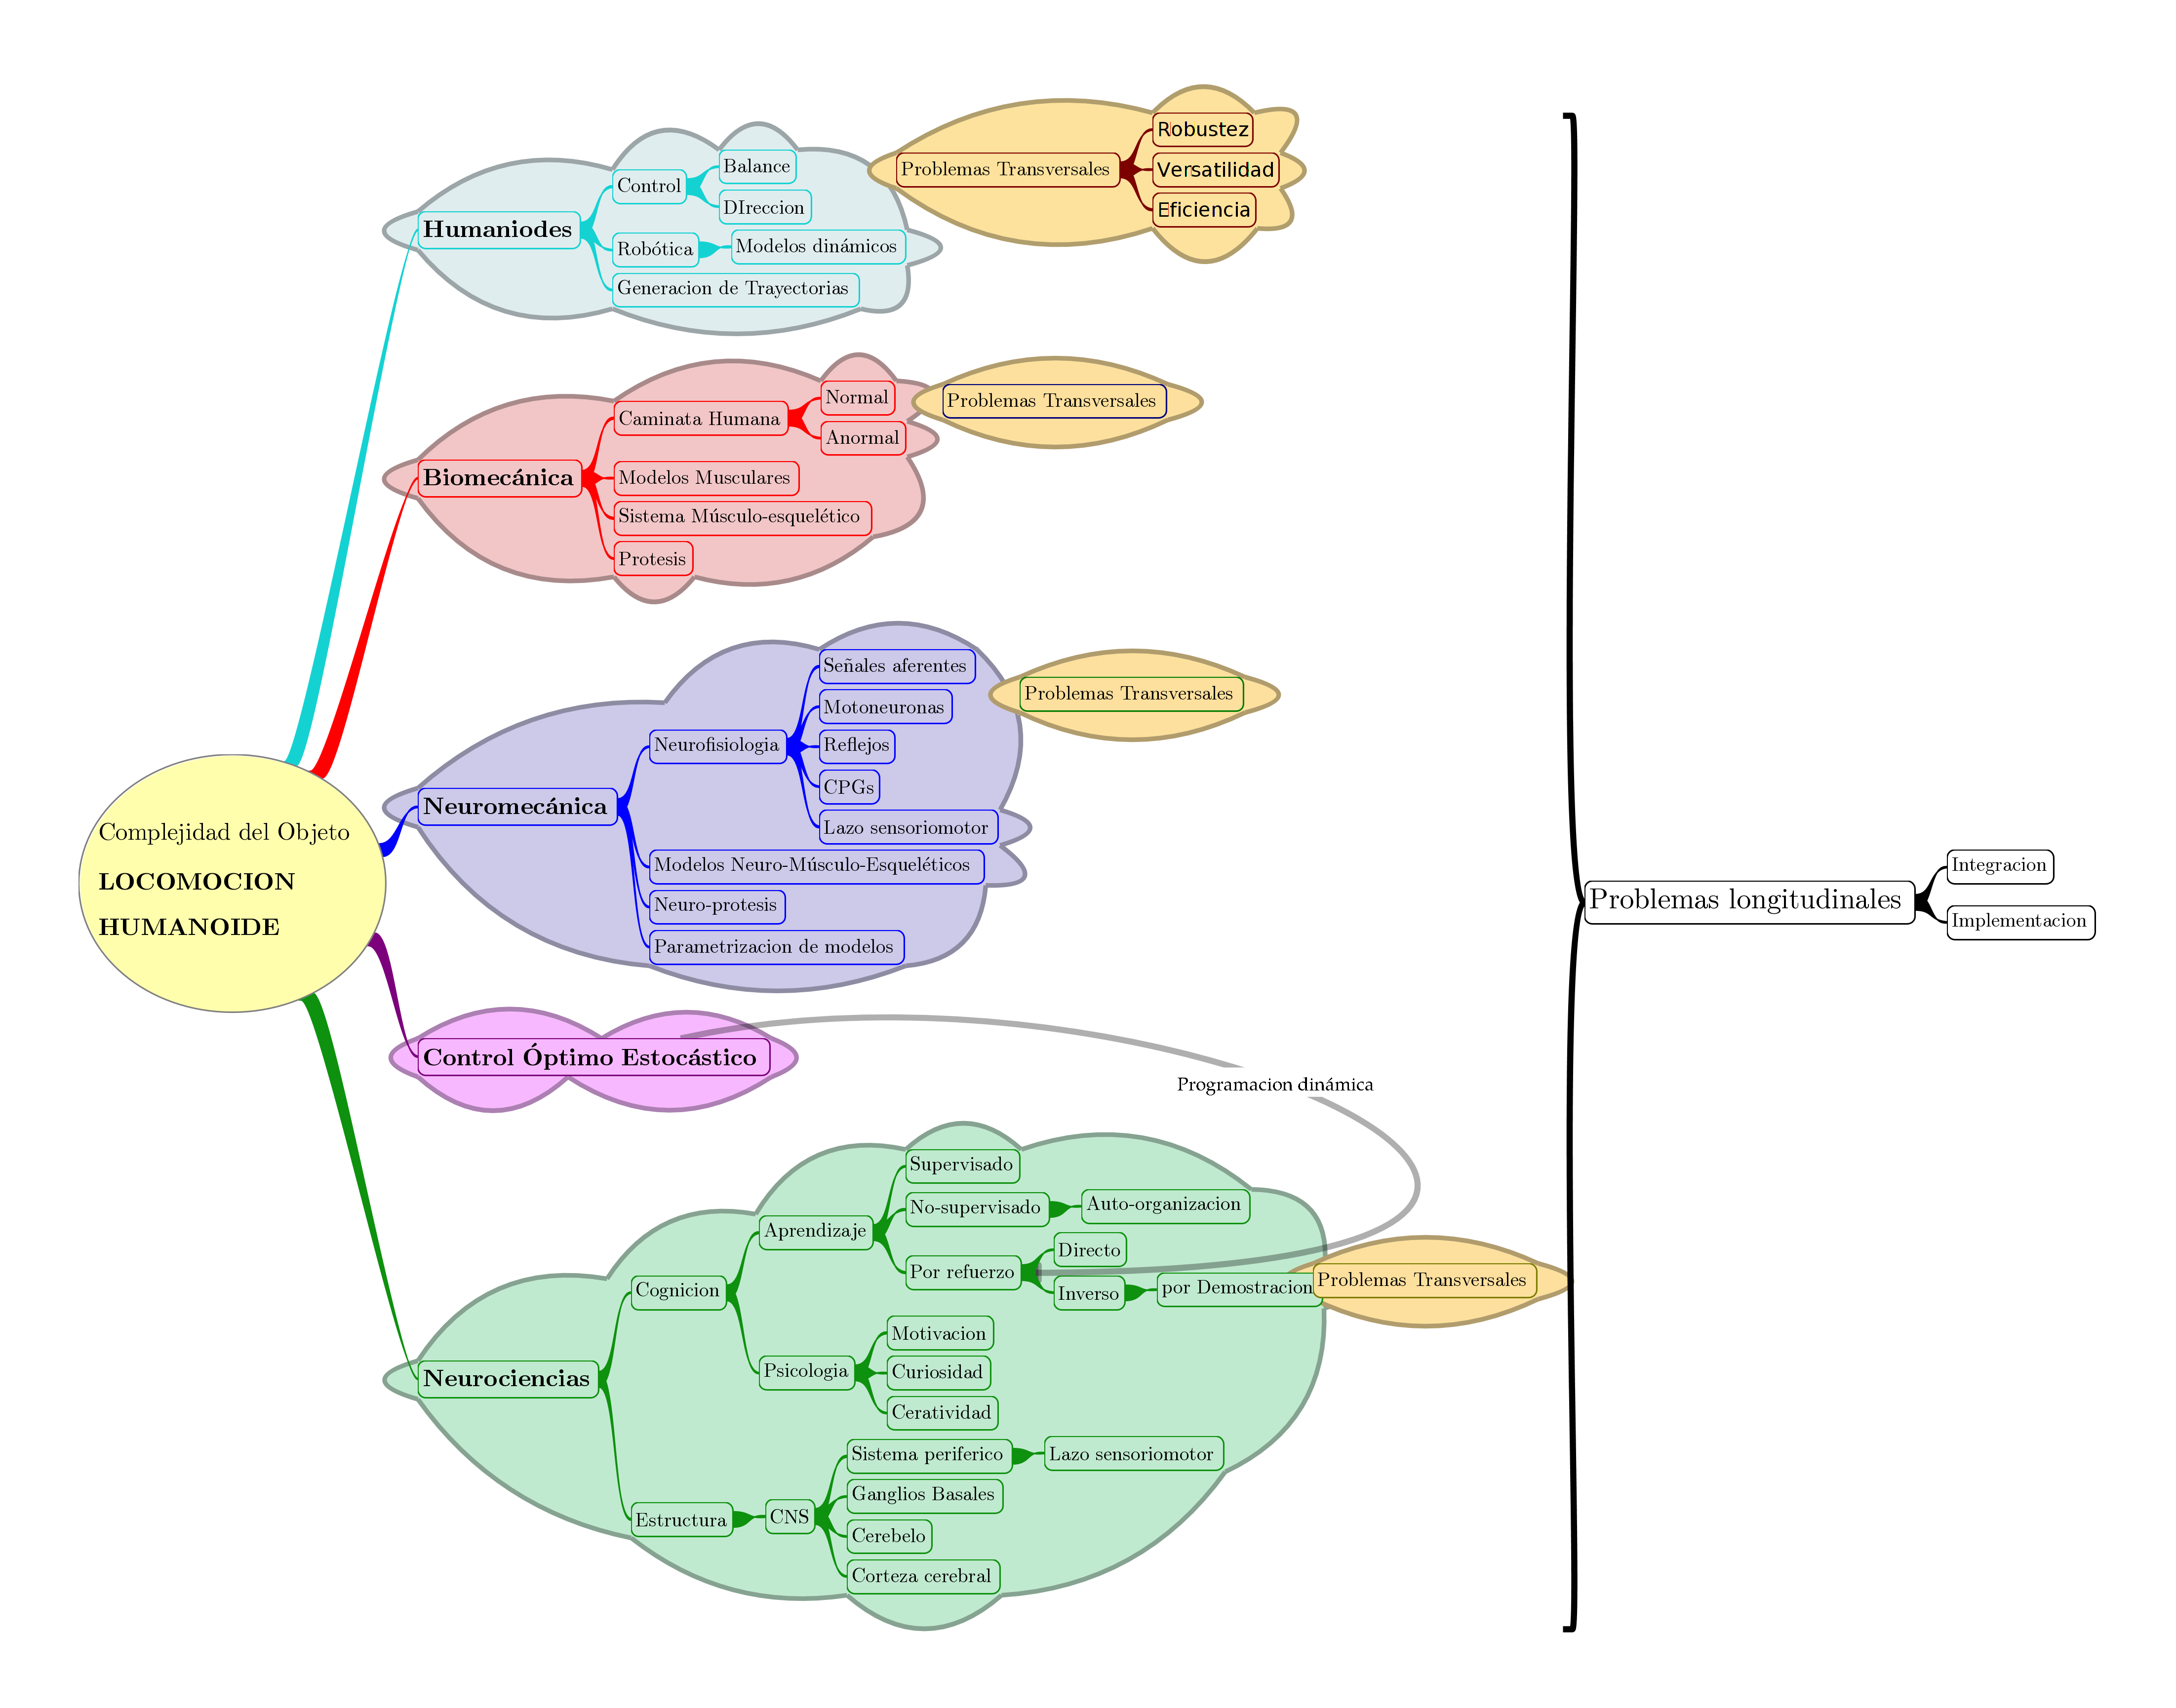
\includegraphics[scale=1.6]{./images/ComplejidadDelObjeto.png}
    \caption{Complejidad del Objeto de inter�s}
    \label{fig:complejidad}
  \end{figure}
\end{landscape}

De la biomec�nica, en el caso de la marcha humana y de la necesidad de biom�mesis~\cite{Ren2014a}, se ha tomado la descripci�n cualitativa de la marcha, descomponi�ndola en fases y eventos que la describen~\cite{Perry2010}. Esta descripci�n es una fuerte fuente de extracci�n de caracter�sticas manual, que permite modelar y proponer leyes de control basada en la cinem�tica y din�mica de la marcha humana para que el humanoide pueda replicar~\cite{Kuo2007a}. El trabajo de~\cite{Kuo1999,Kuo2002}, que eval�a por separado la actuaci�n del tobillo, la cadera y el balance del torso, es un trabajo altamente relacionado con la marcha humana, una de las principales hip�tesis, \emph{los seis determinantes}~\cite{Saunders1953}, sobre los cuales se plantean hip�tesis puramente mec�nicas del almacenamiento y liberaci�n de la energ�a, han sido fundamentales para trabajos recientes en el �rea~\cite{Collins2009,Collins2010,Kuo2010,Huang2015,Riddick2016,Wu2016}.

En la neuromec�nica, la fisiolog�a de los m�sculos y el sistema neuronal perif�rico es descrito como parte del lazo sensorio-motriz, que conforma el canal de comunicaci�n entre el control cerebral y el mundo externo para su movimiento~\cite{McMahon1984}. Modelos de m�sculos y redes neuronales como el caso de los modelos musculares de Hill~\cite{Geyer2006,Haeufle2012}, las redes o ``pathways'' de reflejos~\cite{Geyer2006,Manoonpong2007,Haeufle2012} y los \emph{Generadores de patrones centrales} CPGs~\cite{Hooper2001,Ijspeert2008}, son pr�stamos de la neuromec�nica, que han sido utilizados en la rob�tica no solo para la dise�o de controladores bio-inspirados virtuales neuromusculares~\cite{Batts2015} y generaci�n de la locomoci�n coordinada de humanoides~\cite{Righetti2006b,Righetti2006} y �nimats~\cite{Buchli2006} mediante CPGs, sino tambi�n devolviendo el pr�stamo al validar hip�tesis neuromec�nicas, al proponer modelos neuro-m�sculo-esquel�ticos humanos~\cite{Song2015,Sharbafi2016}, mejorando y proponiendo nuevas teor�as de locomoci�n sin la necesidad de la experimentaci�n \emph{in-vivo}~\cite{Dzeladini2014,Noot2015}, como sucedi� en el comienzo del siglo XX para comprobar hip�tesis de locomoci�n entre reflejos y CPGs con animales~\cite{Manoonpong2007a}. Esto coloca la rob�tica como una herramienta para la biolog�a~\cite{Ghigliazza2004,Proctor2010,Blumberg2013} y la neuromec�nica~\cite{Eilenberg2009,Eilenberg2010,Thatte2015} para probar hip�tesis del desarrollo de la locomoci�n~\cite{Doncieux2015}, mediante pruebas \emph{in-silico}, un ejemplo de ello son~\cite{Marques2014,Dzeladini2014}.

Con el estudio y desarrollo de los caminadores PWD~\cite{Collins2005}, donde se comprob� que un oscilador mec�nico en ausencia de control e interactuando con su entorno~\cite{McGeer1990}, logra una caminata estable~\cite{Thuilot1997}. Y posterior a esto, con las ideas de inteligencia encarnada~\cite{Pfeifer2007}\footnote{Materializado y/o corporalizado, embodiment embodied}, el concepto de computaci�n y control morfol�gico surgi�~\cite{Fuchslin2013}, estableciendo la idea principal como delegar parte del c�mputo requerido por el control central, es decir el cerebro, a la morfolog�a del humanoide~\cite{Hauser2012} y con ello una mayor explotaci�n de la din�mica natural y el lazo sensorio-motriz. En este punto las investigaciones se dirigieron a: (1) la auto-organizaci�n de los reflejos y circuitos a partir de la informaci�n del lazo sensorio-motriz utilizando la teor�a de la informaci�n~\cite{Martius2014} y el uso de redes neuronales artificiales~\cite{Marques2013,Marques2014,HauserS2013}, (2) el beneficio de usar las no-linealidades del sistema neuro-m�sculo-esquel�tico, como la simplificaci�n de las se�ales de control cerebrales~\cite{Ghazi-Zahedi2015}, (3) la riqueza din�mica de atractores peri�dicos y singulares presentes en los arreglos estructurales neuro-m�sculo-esquel�tico como fuente de c�mputo y representaci�n de modelos din�micos internos del entorno y su interacci�n~\cite{Iida2006,Iida2008,Iida2009,Hauser2012a}. Y (4) la parametrizaci�n del sistema neuro-m�sculo-esquel�tico mediante algoritmos evolutivos~\cite{Geyer2003,Song2015,Geyer2010}, bioinspirados~\cite{Dzeladini2014,Noot2015,Kim2009,Li2015} y aprendizaje por refuerzo~\cite{Chu2008,Nakamura2007,Li2013a,Li2014} fueron la herramienta que tom� la rob�tica evolutiva para estudiar, dise�ar, desarrollar y buscar la emergencia de comportamientos en humanoides desde un punto de vista no simplificado e integral buscando las sinergias del conjunto, enfoque que es diametralmente opuesto con los procesos de dise�o ingenieriles frecuentemente empleados, en los que se estudia el problema usando subsistemas aislados y mediante modelos simplificados~\cite{Doncieux2015}.

As� pues la neuromec�nica dejo nuevos problemas en el estudio del movimiento coordinado y entonces nuevas t�cnicas y m�todos fueron necesarios para continuar el estudio de la locomoci�n humanoide~\cite{Buschmann2015}. Las neurociencias integrando teor�as de aprendizaje y desarrollo provenientes de la  psicolog�a y la neurobiolog�a~\cite{Arbib2003,Mirolli2011,Baldassarre2013} formaron nuevas esperanzas, formando estructuras funcionales rob�ticas que intentan imitar la estructura del \emph{sistema nervioso central} CNS, constituida por regiones como: la corteza cerebral~\cite{Dasgupta2014}, el cerebelo~\cite{Dasgupta2014}, el t�lamo~\cite{Jordan2014,Mart2012}, el tronco cerebral~\cite{Santos2011,Or2009}, los ganglios basales~\cite{Grillner2008,Haith2013,Dasgupta2014} y la regi�n mesencef�lica de locomoci�n~\cite{Shahbazi2012}. �stas teor�as, las cuales han sido implementadas con modelos sencillos por la \emph{Inteligencia Artificial} (AI), han utilizando redes neuronales artificiales las cuales pueden aprender y memorizar~\cite{Schmidhuber2015} utilizando simples reglas de aprendizaje, que representan la plasticidad de la neurona biol�gica mediante modelos matem�ticos como las reglas de Hebb y otras reglas~\cite{Der2015} que han permitido esquematizar el aprendizaje en tres grandes vertientes~\cite{Russell2003}: (1) supervisado, (2) no-supervisado y (3) por refuerzo. En los dos primeros las reglas sin�pticas son comprobadas. En el segundo los fen�menos de auto-organizaci�n y extracci�n de caracter�sticas se hacen presentes. Y en el tercer caso, el cual es el que hoy en d�a se estudia con mayor intensidad, convergen nuevas teor�as y esfuerzos provenientes de la psicolog�a, el aprendizaje de m�quina, la teor�a de la informaci�n, la neurobiolog�a y el control �ptimo estoc�stico, integrando as� caracter�sticas cognitivas nuevas al desarrollo de los humanoides~\cite{Schack2009,Polani2011,Kurup2012,Schack2013,Maniadakis2014}.

El aprendizaje por refuerzo RL, proveniente de las teor�as de comportamiento condicional de Pavlov~\cite{Lewis2009,Khan2012}, se ha constituido muy bien en la AI, espec�ficamente con buenos resultados en ambientes donde los agentes realizan acciones finitas en cada estado y la dimensi�n del espacio estado-acci�n es peque�a~\cite{Busoniu2010a,Xu2014}. En casos continuos, el planteamiento se asemeja a los problemas encontrados en el control �ptimo~\cite{Kappen2005,Lewis2009,Khan2012} y el problema ha requerido de t�cnicas m�s elaboradas como la b�squeda de pol�ticas\footnote{Los m�todos de \emph{policy search} (PS)} o de ``leyes de control''~\cite{Grondman2012}, utilizando las t�cnicas de optimizaci�n basadas o no en gradiente~\cite{Gomez2014}. Generalmente se utilizan bases de funciones, usualmente ANNs o FIS~\cite{Wang2007}, como aproximadores para enfrentar el problema de la dimensionalidad~\cite{Zhou2002,Busoniu2010a}. Otro m�todo para enfrentar este problema son los \emph{mejoramientos de pol�ticas empleando integrales de trayectoria} $PI^2$~\cite{Kober2014}. La cantidad de algoritmos propuestos para control utilizando RL, han requerido al igual que en las t�cnicas de optimizaci�n, de la normalizaci�n de Benchmarks para su validaci�n~\cite{Riedmiller2007,Wulfmeier2015,Duan2016}. Un humanoide simulado, representado por una cadena cinem�tica multicuerpo, que por su gran n�mero de grados de libertad ha sido adoptado en recientes Benchmarks como una de las pruebas est�ndar para la maldici�n de la dimensionalidad se puede encontrar en~\cite{Duan2016}.

Otro problema del RL, el dilema de la exploraci�n-explotaci�n, el cual es importante en la velocidad de aprendizaje y la b�squeda de �ptimos globales. Ha sido inicialmente atacado con heur�sticas como \emph{$\epsilon$-greedy} o distribuciones de Boltzmann~\cite{Sutton1998}. Sin embargo las nuevas tendencias imitando mecanismos de curiosidad~\cite{Frank2014} y motivaci�n intr�nseca~\cite{Oudeyer2009}, utilizando la maximizaci�n de la informaci�n~\cite{Ay2012}, las redes bayesianas~\cite{Calandra2016} y aplicando nuevas reglas de plasticidad~\cite{Der2015,Dasgupta2015,Grinke2015} con el fin de la formaci�n de modelos predictivos internos~\cite{Martius2014,Dzeladini2014,Calandra2015,Calandra2016}, han sido propuestas y estudiadas dando mejores resultados. Aunque la mayor�a de �stas no han sido probadas o implementadas en locomoci�n b�peda humanoide, sino m�s bien a la manipulaci�n de objetos~\cite{Frank2014}, se cree, ac�, que estas podr�an acelerar el aprendizaje de la locomoci�n gruesa humanoide, tal como lo es la caminata.

Finalmente, uno de los m�s importantes es el dise�o de la se�al de recompensa, sobre la cual se codifica el comportamiento o estrategia de control del humanoide para desempe�ar una tarea espec�fica. Sobre esta idea se plantea el \emph{aprendizaje por refuerzo inverso} (IRL)~\cite{Mombaur2010} que es muy parecido al problema de control �ptimo inverso~\cite{Kappen2005,Lewis2009,Park2010}, del cual se desprende y soluciona el aprendizaje por demostraci�n~\cite{Pastor2009,Deisenroth2012} y el control por objetivos jer�rquico~\cite{Schack2013,Kober2013}. El principal problema del dise�o o escogencia de la se�al de recompensa, ya sea en directo o inverso del aprendizaje por refuerzo, es la necesidad de imponer diferentes caracter�sticas a mano, que traten de describir el problema u objetivo lo mejor posible. Recientemente la utilizaci�n de las redes profundas ha sido utilizada para la extracci�n de caracter�sticas de forma autom�tica en numerosos problemas de extracci�n de patrones como el procesamiento de im�genes, que permite de forma auto-organizada reproducir el comportamiento coordinado presente en los humanos directamente en los humanoides y agentes virtuales~\cite{Levine2013,Wulfmeier2015,Mnih2015,Duan2016}. Este aprendizaje profundo se ha comenzado a utilizar en la b�squeda de pol�ticas, la representaci�n de modelos gr�ficos y la aproximaci�n de distribuciones de probabilidad (como funciones de: pol�tica, transici�n, recompensa y/o valor) debido a su capacidad de mapeador complejo no-lineal. Y en combinaci�n con la maximizaci�n de la entrop�a~\cite{Wulfmeier2015}, las heur�sticas de exploraci�n se han logrado implementar en plataformas reales.

Dise�ar o encontrar un conjunto de caracter�sticas, al igual que una apropiada morfolog�a, permite reducir la complejidad de la toma de decisiones o el control de una tarea como la locomoci�n b�peda. Este conjunto de caracter�sticas se puede encontrara a mano (por ejemplo ZMP, LIPM o FRI) o mediante algoritmos de \emph{aprendizaje de la representaci�n}, como es el caso de los autoencoders en donde las ideas de auto-organizaci�n son intr�nsecas. En este punto el \emph{Deep Learning} o aprendizaje profundo, es una herramienta del aprendizaje de m�quina que permite el aprendizaje de la representaci�n mediante la construcci�n de una estructura de caracter�sticas o conceptos sencillos, que cada vez se reutilizan para formar conceptos m�s complejos~\cite{Goodfellow2016}.

\section{Situaci�n problem�tica}
\label{sec:problematica}

En la secci�n anterior \ref{sec:complejidad}, se mostr� de forma resumida el camino investigativo del desarrollo de humanoides de forma transversal y longitudinal. Al comenzar a mezclar diferentes �reas del conocimiento, es decir biomec�nica, neuromec�nica, control, inteligencia artificial, neurociencias y psicolog�a, mostrando los avances presentes gracias a cada una de las �reas y etapas, sobre las cuales ha progresado la locomoci�n artificial y donde adem�s se mencionaron los problemas actuales, se puede plantear mejor una panor�mica de los diferentes problemas presentes en la locomoci�n humanoide y de esta forma definir el problema de esta investigaci�n.

De forma global actualmente se busca: 
\begin{quotation}
  \textbf{Problema General:} \emph{Lograr la encarnaci�n de la inteligencia a un sistema rob�tico humanoide, sobre el cual emerja la capacidad de ser aut�nomo, auto-organizado, vers�til, robusto y eficiente, en donde se pueda asignar tareas u objetivos de forma sencilla, sin la necesidad de programarlo al detalle mediante algoritmos y lenguajes complejos},
\end{quotation}
Es la problem�tica general sobre la cual se pretende aportar en la propuesta de este documento y en donde comienza la definici�n del objeto de investigaci�n.
 
No obstante este objeto investigativo debe ser descrito mejor, acotando y delimitando a un caso espec�fico que ser� centrado en:
\begin{quotation}
  \textbf{Problema Detallado y Reducido:} \emph{Lograr una locomoci�n b�peda coordinada, emergente, vers�til, robusta, eficiente y aut�noma de una estructura b�peda humanoide incluyendo una inteligencia encarnada, un lazo sensorio-motor neuromuscular y sus extremidades superiores,
  capaz de:
  \begin{itemize}
  \item Satisfacer tareas u objetivos requeridos por el humanoide, los cuales implican desplazarse en su entorno mediante su propia motivaci�n intr�nseca o curiosidad, tomando as� sus propias decisiones.
  \item Optimizar sus movimientos dependiendo seg�n sean sus necesidades, como por ejemplo: reducir tiempo, reducir energ�a o tan solo llegar al objetivo final, como una meta o realizar una funci�n de movimiento.
  \item Aprender por medio de demostraciones, de forma que le permita adquirir modelos del mundo que lo rodea, sin la necesidad por parte del dise�ador de programarle de forma compleja y detallada, permitiendo de esta forma acelerar su aprendizaje.
  \end{itemize}}
\end{quotation}
Explicando un poco m�s la problem�tica detallada y reducida, en cuanto a la \emph{emergencia de los comportamientos coordinados}, el lazo sensorio-motor ha mostrado tener la capacidad de encarnar fen�menos de auto-organizaci�n~\cite{HauserS2013,Marques2014,Marques2013} que guiados por la organizaci�n de la informaci�n que fluye a trav�s de �l~\cite{Ay2014,Ay2015}, concluye en comportamientos emergentes coordinados~\cite{Der2015,Nurzaman2015,Kim2015}, que pueden codificar comportamientos que ya no requieren de construcciones de alto nivel cognitivo como la motivaci�n o la curiosidad~\cite{Der2015}. En cuanto a la \emph{autonom�a}, la redundancia de tener el lazo sensoriomotor, los mecanismos de motivaci�n y curiosidad explorar�n este punto~\cite{Ay2012}. Y en cuanto al \emph{uso de las extremidades superiores}, mediante la exploraci�n de la din�mica natural, �stas se utilizan para diferentes fines relacionados con la \emph{motricidad gruesa}: (1) reducir el espacio de b�squeda, (2) ayudar al balance y equilibrio, (3) gateo, (4) ponerse de pie~\cite{Der2012,Martius2010}. Para lo que NO se usan en esta investigaci�n los brazos es para manipulaci�n y agarre de objetos, es decir para tareas de \emph{motricidad fina}.

El problema global, es que las estrategias de locomoci�n humanoide tradicionales, son muy limitadas en versatilidad, robustez y eficiencia en su conjunto~\cite{Boer2012}. Adem�s requieren de mucha programaci�n y esfuerzo ingenieril para su realizaci�n, sin dejar de lado la necesidad de la definici�n de un ambiente estructurado que reduzca las incertidumbres que enfrenta el humanoide. Para esto, una soluci�n se cree que es dotar al humanoide de mecanismos con redundancia que promuevan la robustez, basados en autonom�a y en explotaci�n de su propia din�mica natural, es decir, al explotar su morfolog�a y lazo sensoriomotor, se permitir� la formaci�n de modelos internos y la capacidad de auto-estructurar el entorno por medio de ellos mismos. Esta soluci�n ha conducido a diversos nuevos problemas m�s puntuales a nivel transversal y longitudinal (ver figura \ref{fig:complejidad}). A nivel transversal, las soluciones trabajan sobre una �nica �rea en profundidad, es decir por ejemplo, en la parte biomec�nica los trabajos de Art Kuo~\cite{Huang2015,Riddick2016,Wu2016}, en donde se investiga las incidencias mec�nicas y energ�ticas de diferentes partes del cuerpo humano en el desempe�o de la caminata desde un enfoque p�ramente biomec�nico. A nivel longitudinal, los trabajos neuro-musculo-esquel�ticos~\cite{Song2015,Batts2015,Thatte2015,Marques2014,Dzeladini2014,Noot2015}, involucran no todas pero si, varias �reas, logrando profundizar en el conjunto de la locomoci�n humanoide, en donde se buscan aportes en cada �rea relacionada.

En esta propuesta, el aporte se intentar� en forma longitudinal, al construir una herramienta que aporte en problemas puntuales, utilizando soluciones parciales ya propuestas de: la autonom�a, la auto-organizaci�n, el lazo sensoriomotor, la computaci�n morfol�gica, la motivaci�n intr�nseca y la curiosidad, para dar dos soluciones, primero, la \emph{extracci�n de caracter�sticas naturales de la locomoci�n b�peda} que propongan nuevas estrategias jer�rquicas de control y nuevos dise�os de humanoides, que se desarrollen de tareas u objetivos simples a objetivos cada vez m�s complejos y que adem�s pueda simplificar o explicar mejor las descripciones biomec�nicas de la marcha humana, y segundo, la \emph{formaci�n de modelos internos del entorno y su interacci�n}, con el objetivo de auto-estructurar el entorno y predecir resultados ante posibles acciones, que permitan acelerar el proceso de aprendizaje mediante \emph{ensayos mentales}\footnote{Mental rehearsal}.

\begin{quotation}
  \textbf{Problema Planteado:} \emph{Lograr una locomoci�n humanoide, similar a la propuesta en ``el problema detallado y reducido'', en donde se pueda puntualmente estudiar a trav�s del flujo de la informaci�n entre el ``entorno-cerebro'', la posibilidad de: (1) extraer caracter�sticas naturales de locomoci�n y (2) la formaci�n de modelos internos que auto-estructuren el entorno y su propio comportamiento.}
\end{quotation} 

\section{Generaci�n de preguntas}
\label{sec:genpreguntas}

Descrita la complejidad del objeto de investigaci�n, en donde se resumen las �reas involucradas con la locomoci�n gruesa del humanoide y los principales problemas presentes de forma transversal y longitudinal, se procedi� a enunciar un problema detallado y reducido, en el cual se describe limitando y detallando un poco m�s el objeto de investigaci�n. Posterior a eso, se enuncia un problema m�s puntual de esta investigaci�n, en el que se pretende utilizar la \emph{extracci�n de caracter�sticas} y la \emph{representaci�n}, para la encarnaci�n de controladores que permitan la emergencia de comportamientos y por ende la autonom�a de un humanoide, bio-inspirado por el sistema neuro-m�sculo-esquel�tico y el sistema nervioso central humano, del cual se espera lograr robustez, versatilidad, eficiencia y un reducido esfuerzo de programaci�n del humanoide. 

Para generar la pregunta, ahora se define unas proposiciones, que luego de observar lo que se hace actualmente, se consideran posibles: 
%Sobre el problema detallado y reducido, y la complejidad del objeto de investigaci�n, en donde se describe las �reas relacionadas, como se describi� anteriormente, para el desarrollo de la motricidad gruesa en la locomoci�n humanoide. Y luego de observar lo que se hace actualmente, se plantea las siguientes proposiciones tom�ndolas como verdaderas:

\begin{quotation}
  \textbf{Proposici�n 1.} \emph{Es posible proponer locomociones artificiales, optimizadas
  localmente sobre la exploraci�n y explotaci�n del lazo
  sensoriomotor, la morfolog�a y el entorno, al utilizar las t�cnicas
  ya conocidas (como la de caminata humanoide empleando ZMP, FRI, IPM,
  CP, HZD), como punto de partida de ejemplos demostrativos de
  locomoci�n, no necesariamente �ptimos pero s� admisibles.}
\end{quotation}
\begin{quotation}
  \textbf{Proposici�n 2.} \emph{Es posible utilizar locomociones artificiales optimizadas 
  para excitar el lazo sensoriomotor con el fin de extraer
  caracter�sticas naturales de locomoci�n.}
\end{quotation}
\begin{quotation}
  \textbf{Proposici�n 3.} \emph{Es posible a partir de las
  caracter�sticas naturales de locomoci�n,
  crear un dise�o del sistema controlador y
  generador de la locomoci�n humanoide.}
\end{quotation}
\begin{quotation}
  \textbf{Proposici�n 4.} \emph{Es posible a partir de las
  caracter�sticas naturales de locomoci�n, explorar distintas formas
  coordinadas de locomoci�n basadas en objetivos impuestos al humanoide, 
  sin la necesidad de estructurar de forma previa el
  entorno para el humanoide.}
\end{quotation}
\begin{quotation}
  \textbf{Proposici�n 5.} \emph{Es posible a partir de las
  caracter�sticas naturales de locomoci�n, formar distintos modelos 
  de la interacci�n del humanoide con su entorno, 
  que permitan la predicci�n del efecto de sus acciones y descripci�n de la estructura del entorno, 
  logrando una auto-estructuraci�n del entorno y sus acciones,
  sin la necesidad de estructurar de forma previa el
  entorno para el humanoide.}
\end{quotation}
Las proposiciones anteriores ser�n utilizadas para el planteamiento de la pregunta de investigaci�n, la formulaci�n de la hip�tesis y la exposici�n de los trabajos relacionados directamente con el problema en la secci�n de los antecedentes.

%�Es posible proponer locomociones artificiales, optimizadas localmente sobre la exploraci�n y explotaci�n del lazo sensoriomotor, la morfolog�a y el entorno, al utilizar las t�cnicas ya conocidas (como la de caminata humanoide empleando ZMP, FRI, IPM, CP, HZD), como punto de partida de ejemplos demostrativos de locomoci�n, no necesariamente �ptimos pero s� admisibles, sobre los cuales se pueda excitar el lazo sensoriomotor para extraer caracter�sticas, que mediante la b�squeda de nuevas pol�ticas permitan: (1) crear un mejor dise�o del sistema controlador y generador de la locomoci�n humanoide, (2) explorar distintas formas coordinadas sin la necesidad de estructurar de forma previa el entorno para el humanoide?

Pero de forma puntual se formula la siguiente pregunta:
\begin{quotation}
%  \textbf{Pregunta de investigaci�n} \emph{�C�mo analizar y organizar la informaci�n procedente de la comunicaci�n a trav�s del lazo sensoriomotor entre el ``entorno-cerebro'', de forma tal, que se pueda extraer ``caracter�sticas naturales de locomoci�n'' y la formaci�n de modelos que auto-estructuren el entorno y su propio comportamiento, permitiendo una reducci�n de la programaci�n en el dise�o y control de humanoides asegurando la emergencia de comportamientos b�pedos en ambientes no estructurados?}
\textbf{Pregunta de investigaci�n} \emph{�C�mo analizar y organizar la informaci�n procedente de la comunicaci�n entre el entorno y el cerebro a trav�s del lazo sensoriomotor, de forma tal, que se pueda extraer caracter�sticas naturales de locomoci�n y la formaci�n de modelos que auto-estructuren el entorno y su propio comportamiento, permitiendo una reducci�n de la programaci�n en el dise�o y control de humanoides asegurando la emergencia de comportamientos b�pedos en ambientes no estructurados?}
\end{quotation}

% La generaci\'on de trajectorias debe emerger de un proceso de adaptaci�n de la estructura mec\'anica a realizar una tarea espec\'ifica. Por ejemplo, la rotaci�n del pie debe emerger de la exploraci\'on y explotaci\'on del desarrollo de habilidades. 
% El control multiestrategias prevee de redundancia al sistema de actuaci\'on o motor. Por ejemplo, la computaci�n morfol�gica y las redes neuronales recurrentes en reservorio, incluyen redundancia al sistema sensorial y de control. Otros ejemplos, son la sobreactuaci�n presente en el sistema musculo-esqueletico o la actuacion de tobillos, torso y cadera.
% La explotaci\'on de habilidades debe conducir a la eficiencia energ\'etica y de otros criterios.
% La adaptacion implica aprendizaje. El desempe\~no de una tarea aprendida requiere de auto-evaluaci\'on, lo que da la posibilidad de usar las hipotesis de motivacion intriseca, que a su vez lleva a la exploracio y explotacion de politicas de control.

% Algunas de las caracter\'isticas de cognici\'on rob\'oticas deseables ser\'ian: Aprendizaje, memoria, razonamiento, planeaci\'on, predicci\'on, acci\'on, comunicaci\'on, atenci\'on, conciencia del tiempo, motivacion y creatividad. Funciones cognitivas inconcientes y Funciones cognitivas concientes (Razonamiento, planeaci\'on y comunicacion)

% ¿Es posible obtener adaptaci\'on y aprendizaje al modular los reflejos existentes por una capa de control superior y adem\'as crear nuevos reflejos?

% ¿C\'omo se pueden formar los reflejos en el agente?

% ¿C\'omo crear estrategias y como se codifica? ¿C\'omo implementar inferencias?

% En la etapa de desarrollo, la b\'usqueda de diferentes habilidades, de forma auto-organizada (Iida y Marques) para actividades como: patalear, rodar en el plano, sentarse, gatear, pararse, caminata est\'atica, caminata din\'amica y correr asi como comportamientos que no se codifican con reflejos y requieren de planeaci\'on de movimientos pero que si necesitan del uso de reflejos. Se requiere de Aprendizaje por refuerzo en la b\'usqueda de p\'oliticas que permitan ajustar el control del agente para lograra una habilidad determinada. 

% El aprendizaje por refuerzo es costos para el agente ya que tiene que experimentar en su entorno para llenarse de conocimiento y aprender nuevos comportamientos. Sin embargo con el conocimiento ya ganado, la representaci\'on de modelos de direntes situacinoes(problemas) le permiten predecir el efecto de sus acciones sobre el estado del cuerpo y entorno en determinado momento para de esta forma poder tomar la mejor decisi\'on en el momento de tomar acci\'on, evitando asi tener que probar de forma f\'isica. De esta forma la predicci\'on y planeaci\'on entran a ser parte de las cualidades cognitivas necesarias para el agente.

% En la parte mas elevada, el razonamiento probabil\'istico debe ser integrado para que el an\'alisis de modelos infiera resultados racionales para la toma de decisiones del agente.

% Autocalibraci\'on de los actuadores, con twitches, que define los l\'imites de fuerza individuales. Autocalibraci\'on de los sensores, de fuerza, elongaci\'on, posici\'on, velocidad, etc,. B\'usqueda de movimientos coordinados, optimizando energ\'ia (Alejarse, acercarse, dirigirse). Codificaci\'on de reflejos b\'asicos y formaci\'on de diferentes movimientos coordinados reflexivos de giro y sentado. Formaci\'on de conceptos de equilibrio. Formaci\'on de equilibrio en dos pies.

% El aprendizaje por refuerzo se puede ver como una motivaci\'on sobre el agente, dicha motivaci\'on puede ser de car\'acter extr\'insico o intr\'insico.

% Los reflejos pueden ser de dos fomras: codificados desde el nacimiento y construidos mediante planeaci\'on, repeticion y optimizaci\'on de la tarea. Ademas, segun su utilidad debn ser heredados a sus descendientes, por lo tanto deben ser codificados en su ADN y por lo tanto deben modificar su genotipo y a su vez su fenotipo. ¿C\'omo se codifican los reflejos en el genotipo? ¿Que lleva a aumentar tama\~no del genotipo?

% En el aqui y el ahora,
% ¿C\'omo y cu\'ales son el conjunto de reflejos b\'asicos que necesita conocer un agente rob\'otico b\'ipedo, para lograr la emergencia de locomoci\'on al nivel del control humano?

% En la etapa ontogen\'etica,
% ¿Cu\'ales son los mecanismos de predici\'on y planeaci\'on que debe tener el agente rob\'otico para una adecuada adaptaci\'on y una generaci\'on robusta de habilidades requeridas por su entorno y que a su vez permita la formaci\'on de reflejos?

% En la etapa filogen\'etica,
% ¿Cu\'ales son las caracter\'isticas morfol\'ogicas y de control que deben evolucionar, para crear dise\~nos rob\'oticos que exploten al l\'imite las tecnolog\'ias actuales?

\section{Hip�tesis}
\label{sec:hypothesis}

La siguiente proposici�n se plantea como posible soluci�n o respuesta al problema de investigaci�n planteado anteriormente:
\begin{quotation}
  \textbf{Formulaci�n de la Hip�tesis} \emph{Utilizar un lazo sensoriomotor, basado en un modelo
  neuro-m�sculo-esquel�tico de un humanoide, permite el an�lisis del
  canal de comunicaci�n entre el entorno-cerebro, para la extracci�n
  de caracter�sticas y la formaci�n de modelos predictivos del
  entorno, que promuevan la auto-estructuraci�n de sus acciones y por ende una 
  reducci�n en la programaci�n, en el dise�o y control de humanoides.}
\end{quotation}

Para una mejor explicaci�n de la hip�tesis, esta se descompone en dos partes, (1) un antecedente o causa y (2) un consecuente o efecto. Partiendo de que la hip�tesis es correcta, entonces se tiene,

\begin{quotation}
  \textbf{Antecedente:} \emph{El humanoide consta de un sistema tal
  que utiliza un lazo sensoriomotor, basado en un modelo de
  comunicaci�n entre el entorno-cerebro, para la extracci�n de
  caracter�sticas y la formaci�n de modelos predictivos de entorno.}
\end{quotation}

\begin{quotation}
  \textbf{Consecuente:} \emph{Las acciones del humanoide son
  auto-estructuradas, al proponer modelos internos del entorno y sus acciones, que a su vez permitan la emergencia de comportamiento y disminuyan la cantidad de programaci�n en el dise�o y control de humanoides.}
\end{quotation}
% \section{Objetivos}
% \label{sec:obj}

% \subsection{Objetivo General}
% \label{sec:objGen}
% Proponer el modelo de un control modular por niveles, que permita planear y ejecutar una locomoci\'on emergente, eficiente, robusta y vers\'atil de una estructura humanoide, para desempe\~narse racionalmente de acuerdo a las necesidades y limitaciones de su cuerpo y entorno, a partir de un conjuto de comportamientos cognitivos y reflejos auto-organizados e implementados morfol\'ogicamente.

% \subsection{Objetivos Espec\'ificos}
% \label{sec:objEsp}
% \begin{itemize}
% \item Generar modelos computacionales parametrizables de humaniodes con estructuras morfol\'ogicas y de control, inspiradas sobre modelos neuro-musculo-esqueleticos pero con actuadores rob\'oticos actuales, sobre los cuales se implemente diferentes tipos de movimientos tomados de modelos de locomoci\'on humana.
% \item Implementar sobre el control y la morfolog\'ia modelos de: estimaci\'on, planeaci\'on, estrategia de acciones y toma de decisiones, sobre los cuales emergan, se aprendan, se hagan robustos, se optimicen y codifiquen de forma cognitiva y/o reflexiva comportamientos de locomoci\'on necesarios para la satisfaci\'on de objetivos generados por el cuerpo-entorno.
% \item Optimizar las caracter\'isticas morfol\'ogicas y de control que permitan optimizar los alcances de una configuraci\'on de robot humaniode actual dadas las limitaciones de actuacion y sensado.
% \end{itemize}

% \section{Resultados Esperados}
% \label{sec:results}
% Programacion automatica de comportamientos.



    \chapter{Antecedentes}
\label{chp:ante}

\section{Modelo Neuro-m�sculo-esquel�tico}
\label{sec:modNMS}

Tal vez el modelo del sistema neuro-m�sculo-esquel�tico NMS que m�s impacto ha tenido recientemente, propuesto por~\cite{Geyer2010}, es un modelo desarrollado en MATLAB y SimMechanics, proponiendo una locomoci�n coordinada de la caminata utilizando un conjunto de reflejos, que act�an sobre un conjunto de m�sculos basados en el modelo de Hill propuesto en~\cite{Geyer2003}, donde se estudia la relaci�n fuerza-longitud-velocidad del m�sculo y los diferentes circuitos (o \emph{pathways}) que se pueden estudiar bajo ese modelo. Los m�sculos se organizan formando sinergias musculares~\cite{DAvella2003}, de forma que permiten al sistema esquel�tico: evitar hiperextenciones de las articulaciones, agregar flexibilidad (\emph{Compliance}), evadir el choque con el piso en la etapa de balanceo, reciclar la energ�a en el tal�n y otras. Se utiliza algoritmos gen�ticos (GAs) para la parametrizaci�n del sistema NMS.

Posterior a este modelo, Geyer continu� el modelo esta vez para un sistema tridimensional~\cite{Song2015} a�adiendo nuevos m�sculos y reflejos, en donde emergen distintos comportamientos de marcha en modo de: caminar, correr, aceleraci�n, desaceleraci�n, negociaci�n de pendientes y escalones, giro, y evasi�n deliberada de obst�culos. El controlador es un sistema jer�rquico compuesto por dos niveles, en el primero se almacenan y coordinan los reflejos y en el segundo se controla el posicionamiento del pie. El proceso de optimizaci�n de los par�metros es cambiado por otra t�cnica evolutiva recientemente utilizada como m�todo de b�squeda de pol�ticas directa, denominada \emph{Covariance Matrix Adpatation-Estrategia Evolutiva} CMA-ES~\cite{Hansen2006}.

Paralelo al trabajo de~\cite{Geyer2010,Song2015}, Andr� Seyfarth continuo desde~\cite{Geyer2003}, con un trabajo sobre el modelo muscular y su importancia en la comunicaci�n de las se�ales realimentadas y prealimentadas en la adaptaci�n a un entorno cambiante o con cierto nivel de incertidumbre~\cite{Haeufle2012}. Dentro del canal de comunicaci�n, las se�ales aferentes provenientes de las fibras sensoriales son estudiadas en detenimiento para el caso de un movimiento peri�dico de salto. Los husos neuromusculares como receptores sensoriales, llevan la informaci�n propioceptiva al controlador, estos son: (1) Longitud y velocidad de alargamiento y contracci�n del m�sculo y (2) los \emph{�rganos tendinosos de Golgi} llevan la informaci�n de la fuerza. Este canal es estudiado concluyendo la importancia de cada una de estas se�ales en la estabilidad y control del salto, adem�s de especificar si la realimentaci�n es positiva o negativa.

El siguiente paso de Haeufle, al comprobar que las no-linealidades eran �tiles en el modelo muscular de~\cite{Haeufle2012}, fue cuantificar la informaci�n que flu�a por el canal al mirar que tanto computo deb�a realizar el controlador para lograr una acci�n espec�fica~\cite{Haeufle2014}, para ello utiliz� \emph{la entrop�a de la informaci�n de Shannon}~\cite{MacKay2005}. Ya metido en el campo de la computaci�n morfol�gica compar� tres modelos de robots saltadores simulados al mirar la complejidad del control en cada uno de los tres siguientes casos: (1) modelo no-lineal del m�sculo de Hill, (2) modelo lineal del m�sculo de Hill y (3) motor DC como actuador~\cite{Ghazi-Zahedi2015a}. Otros modelos de m�sculos basados en Hill son propuestos en~\cite{Schmitt2015} complementan mejor la comparaci�n de un control real.

Extendiendo el trabajo de~\cite{Geyer2010} y paralelo a~\cite{Song2015}, Auke Ijspeert, conocido por su trabajo en CPGs~\cite{Ijspeert2008}, muestra la necesidad de incluir los CPGs en la estructura puramente reflexiva de Geyer en~\cite{Dzeladini2014}. Aunque el modelo de Geyer es estable en presencia de perturbaciones, la modulaci�n de la velocidad y el tama�o del paso no son problemas sencillos y requieren de procesos de optimizaci�n \emph{offline} demorados. Al incluir los CPGs en el modelo NMS, la modulaci�n de la velocidad y el paso de la marcha se tornan sencillas y adem�s se muestra que los CPGs pueden ser utilizados como modelos predictivos del lazo sensoriomotor, al ser capaces de reproducir las se�ales aferentes generadas por una marcha estable. Esta capacidad predictiva de los CPGs ofrece una forma de comparar la importancia relativa de distintos circuitos o pathways de realimentaci�n. Como trabajos futuros, se propone un estudio de co-evoluci�n de las componentes de realimentaci�n y prealimentaci�n. Adicional se concluye que las se�ales de los pathways pueden ser estudiadas mejor a trav�s de las se�ales de las motoneuronas, formando se�ales de baja dimensi�n compuesta por cuatro primitivas motrices controlando con una mayor facilidad la velocidad, longitud de paso, transici�n de marchas y la adaptaci�n a pendientes cambiantes. La reducci�n de dimensionalidad expresada en primitivas de movimiento, de nuevo es estudiada por Ijspeert en~\cite{Sprowitz2014a}, donde se analiza el flujo de informaci�n mediante PCA y se reduce a los cuatro primero componentes logrando un 95\% de precisi�n.

Los CPGs codifican la informaci�n mediante circuitos neuronales~\cite{Grillner1985}, que se pueden analizar mediante diferentes tipos de osciladores aunque el m�s utilizado recientemente es el de Kuramoto. En el trabajo de~\cite{Dzeladini2014}, se utilizan osciladores morfados~\cite{Ajallooeian2013}. La implementaci�n de ~\cite{Dzeladini2014} fue desarrollada en C++, escribiendo unas librer�as para el sistema NMS. La optimizaci�n de los par�metros se llev� acabo con un algoritmo multi-criterio, ya que siempre se emplearon entre dos o m�s criterios. Los criterios principales fueron: minimizaci�n de la energ�a, penalidad por la hiperextensi�n de la rodilla, velocidad y longitud de paso. Se emplearon dos t�cnicas, Ordenamiento Lexicogr�fico para manejar el ordenamiento multiobejetivo de la funci�n de \emph{fitness} sobre el frente de Pareto y la \emph{optimizaci�n basada en enjambres de part�culas} PSO como estrategia de b�squeda principal.

Auke Ijspeert desarrolla un framework en~\cite{Ajallooeian2013}, dirigido al aprendizaje de la locomoci�n, denominado ``osciladores de fase no-lineales morfados''. Esta familia de osciladores incluye a los CPGs y a las primitivas de movimiento din�micas DMPs~\cite{Ijspeert2002,Ijspeert2013} desarrolladas por inicialmente por Stefan Schaal. Esta es otra de las caracter�sticas de la encarnaci�n de la inteligencia utilizando la computaci�n morfol�gica, ya que este framework permite el dise�o de sistemas din�micos con distintos tipos de atractores. Sobre los Osciladores Morfados (MO) se construye una arquitectura Actor-Critica para el aprendizaje de la locomoci�n, compuesto de CPGs y DMPs para movimientos peri�dicos y discretos~\cite{Li2013a,Li2014}. La importancia de los MO radica en la reducci�n de la dimensionalidad, la cual es un problema de escalabilidad presente en el \emph{aprendizaje por refuerzo} (RL), permitiendo utilizar m�todos de b�squeda de pol�tica directa o basada en gradiente como el actor-cr�tico~\cite{DeBroissia2016}.

Otro trabajo sobre la formaci�n de reflejos sin la necesidad de CPGs, es presentado por Fumiya Iida en~\cite{Marques2013,Marques2014}, implementando un esquema de desarrollo intr�nsecamente incremental, en donde prueba cuatro hip�tesis sobre el desarrollo motor, que incluyen~\cite{Marques2014}: (1) a partir de las \emph{actividades motoras espont�neas} (SMA), presentes en el desarrollo fetal de los mam�feros, se puede generar reflejos, (2) que al interactuar con su morfolog�a y entorno se forman de manera auto-organizada, (3) sobre los cuales en una modulaci�n supraespinal de los reflejos, emergen comportamientos coordinados, que por �ltimo (4) demuestra que los tres pasos anteriores siguen estando activos durante el desarrollo y la vida del individuo, al probar aplicando cambios en la morfolog�a con el fin de representar una lesi�n, para posterior a esto mostrar la capacidad de adaptaci�n y robustez del sistema. Una similitud con el trabajo de~\cite{Song2015} a parte del sistema m�sculo-esquel�tico y el modelo de Hill, es la jerarqu�a del controlador, compuesta por dos etapas: pasiva y activa, en la etapa pasiva los reflejos proponen un comportamiento coordinado, pero dicho comportamiento puede ser modulado por la etapa activa mediante se�ales supraespinales. A diferencia del trabajo de Geyer, los reflejos son auto-organizados siguiendo un trabajo previo descrito en~\cite{Marques2013}, en donde la correlaci�n de las se�ales sensoriales y motoras determinan los \emph{pathways} o patrones de conectividad de los diferentes circuitos reflexivos, la etapa pasiva es descrita en este art�culo. En especial se habla de tres reflejos: reflejo de estiramiento, reflejo de inhibici�n rec�proca y reflejo de estiramiento inverso\footnote{stretch o myotatic reflex, reciprocal inhibition reflex, reverse stretch o myotatic reflex}. El proceso de auto-organizaci�n basado en correlaci�n, es un proceso no supervisado utilizando una regla anti-hebbiana conocida como anti-Oja.

Aplicaciones:

(Geyer)
Sobre pr�tesis transfemorales se estudia la recuperaci�n del balance de la marcha utilizando un control NM~\cite{Thatte2015}, logrando una mayor robustez en la marcha comparado con los controladores de impedancia, los cuales se destacan en pr�tesis actuadas. Esta comparaci�n se realiza mediante simulaci�n y hardware, obteniendo como resultado una mejor comunicaci�n entre el usuario y la pr�tesis, pero al final se plantea que es necesario estudiar mejor dicha pol�tica de control analizando la marcha anormal de un amputado.

\cite{Dzeladini2016}(Ijspeert)
Dzeladini, F. et al., 2016. Effects of a neuromuscular controller on a powered ankle exoskeleton during human walking. In Proceedings of the IEEE RAS and EMBS International Conference on Biomedical Robotics and Biomechatronics. pp. 617

\section{Computaci�n morfol�gica y lazo sensoriomotor}
\label{sec:morphComp}

Las ideas de \emph{encarnaci�n de la inteligencia}, planteadas en~\cite{Pfeifer2007}, donde se propone unos principios de dise�o de inteligencia artificial encarnada, mencionan a la \emph{computaci�n morfol�gica} (MC), como uno de los principales dominios de la Inteligencia sobre la Naturaleza, sobre los cuales la vida a trav�s de la evoluci�n y el desarrollo ha perfeccionado su cuerpo, permiti�ndole adaptarse y permitir la emergencia de nuevos comportamientos, sobre los cuales el individuo puede interactuar mejor con el entorno en que subsiste. La alta riqueza no-lineal din�mica que est� presente en el material y la morfolog�a de los seres vivos, es demostrada en trabajos \emph{in-silico} de Fumiya Iida, donde se explora la din�mica natural y el flujo de informaci�n a trav�s del cuerpo encontrado en el sistema m�sculo-esquel�tico~\cite{Iida2008,Iida2006}. 

Helmut Hauser siguiendo a Pfeifer, se plantea una capacidad de c�mputo que es demostrada, realizada por el material y la morfolog�a en~\cite{Hauser2012a,Hauser2012}, aqu� el material y sus propiedades pasa a ser parte de la morfolog�a, que est�n representados por un arreglo aleatorio de resortes no-lineales sobre los cuales se demuestra que por medio de una \emph{salida est�tica}\footnote{static readout: es el nombre utilizado en los art�culos}, la morfolog�a de un individuo es capaz de efectuar c�mputos que involucran varios procedimientos como: cinem�ticas inversas (IK) y directas (DK)~\cite{Li2013a}, din�micas inversas (ID) y directas (DD)~\cite{Hauser2012}, c�lculos multitarea y en paralelo~\cite{Hauser2012}, memorizaci�n de ciclos l�mite~\cite{Hauser2012a,Hauser2014}, memoria a corto plazo~\cite{Nakajima2014}, simplificaci�n de las se�ales de control~\cite{Ghazi-Zahedi2015a} y otras m�s. El computador morfol�gico es definido mediante la existencia de unas propiedades como: (1) \emph{Separabilidad de entrada}, la cual es lograda mediante un mapeo no-lineal entre un espacio de baja dimensi�n a un espacio de alta dimensi�n, como en el m�todo de las \emph{m�quinas de soporte vectorial}. (2) \emph{Memoria desvaneciente} que consiste en sostener o mantener una secuencia de entrada reciente en el sistema, la cual permite integrar la informaci�n de los est�mulos a trav�s del tiempo sobre la parte importante de la se�al, esta propiedad es explorada en~\cite{Nakajima2014}.

El trabajo de Hauser es soportado matem�ticamente y fundamentado en (1) los sistemas din�micos, (2) el control no-lineal realimentado y (3) la capacidad de c�mputo, la relaci�n de estos fundamentos previamente explicados por~\cite{Maass2007} de las redes neuronales en configuraci�n de \emph{reservorio}, forman parte de un caso de la t�cnica \emph{computaci�n reservorio} del \emph{aprendizaje de m�quina} en donde el aprendizaje se realiza mediante una simple regresi�n lineal~\cite{Hauser2014}. El arreglo de resortes propuesto por Hauser es denominado un \emph{reservorio f�sico} y de forma formal se da una definici�n matem�tica de computaci�n y control morfol�gico reuniendo los trabajos anteriores en~\cite{Fuchslin2013,Hauser2013}, en donde se destacan diferentes aplicaciones de biomec�nica y medicina utilizando la mec�nica cl�sica y la mec�nica estad�stica.

La \emph{morfosis} o \emph{morfolog�a adaptativa}~\cite{Hauser2017}, es el concepto m�s reciente que se estudia en MC, mediante esta propiedad del sistema, el cambio de los par�metros que definen la morfolog�a permiten el cambio de atractores din�micos, los cuales representan o codifican un determinado comportamiento, sin la necesidad de cambiar la se�al de control. En lugar de cambiar la se�al de control al presentarse un cambio en el entorno, la morfolog�a se adapta logrando configuraciones de comportamientos eficientes cuando el sistema permite la morfosis. Por lo tanto la morfosis permite operar en escenarios ruidosos y proponer investigaciones futuras en estructuras jer�rquicas de control de alto nivel, el crecimiento artificial de la estructura, los sistemas auto-curativos. Las ideas de morfosis fueron implementadas~\cite{Vu2013} en una plataforma rob�tica mono-p�dica basada en un sistema biela-manivela de \emph{actuaci�n rigidez variable} (VSA), inmersa en un ambiente variable de escalones, pendientes y diferentes rugosidades del piso, sobre los cuales el comportamiento de la se�al de control para lograr el movimiento se mantuvo fijo y se exploro los par�metros del mecanismo biela-manivela, sobre el cual comportamientos adecuados para cada configuraci�n del piso y mostrando un desempe�o eficiente. Otra implementaci�n de morfosis es el ya mencionado trabajo de~\cite{Song2015}.

Con los trabajos anteriores se demostr� la presencia de la computaci�n morfol�gica en la locomoci�n y el comportamiento de las especies. Las tendencias de investigaci�n de esta �rea se dirigieron hacia la formaci�n del comportamiento de forma aut�noma por parte del \emph{agente}~\cite{Martius2014}. El car�cter estoc�stico, la auto-organizaci�n y el flujo de informaci�n entre el agente y el entorno son ahora los principales temas estudiados. El problema del MC tom� herramientas del control �ptimo estoc�stico, el aprendizaje por refuerzo y la teor�a de la informaci�n. A continuaci�n se resume algunos trabajos de grupos de investigadores con respecto al �rea de MC y sus nuevos problemas.

Continuando con las ideas de MC~\cite{Pfeifer2007}, en \cite{Ruckert2012} el prop�sito principal es, c�mo cuantificar la cantidad de control que el sistema rob�tico le delega a la morfolog�a. Para esto una cadena serial de cuatro eslabones, es utilizada para modelar el balance de un humanoide aplicando torque en diferentes articulaciones (tobillos, rodillas, cadera y brazos), adem�s el balance se debe mantener en presencia de empujones externos. Los par�metros que forman parte de la morfolog�a, los cuales son explorados son: la fricci�n de articulaci�n, lo longitud de los eslabones e inspirado por el trabajo de~\cite{Hauser2012}, se utilizaron resortes lineales cuyo acople con los eslabones permit�an un comportamiento no-lineal en el torque de la articulaci�n. Se utiliz� CMA-ES para la b�squeda de la morfolog�a. La idea principal es: (1) utilizar el \emph{Control �ptimo Estoc�stico} (SOC) para proponer leyes de control sobre cualquier morfolog�a y (2) a partir de esto cambiar la morfolog�a con el fin de reducir la complejidad de la se�al de control y lograr un alto desempe�o, obteniendo as� un control y morfolog�a �ptimos. 
TODO: INCLUIR: Variaci�n de las ganancias de control y la relaci�n de computo del controlador. El modelo gr�fico y el m�todo AICO.

Martius y Ralf Der con sus playful machines, mencionar el trabajo con Hauser.

Nihat Ay plantea el lazo sensoriomotor mediante un modelo gr�fico (o red bayesiana) causal, en donde los fen�menos estoc�sticos de la interacci�n de un agente y su entorno, pueden ser modelados y las pol�ticas o estrategias de control, pueden ser buscadas mediante el aprendizaje por refuerzo y el control �ptimo estoc�stico pero donde la informaci�n que fluye a trav�s del lazo debe de ser organizada. Modelos de CRBM.

Elmar R�ckert, Calanca y Peters, modelo PMP, redes bayesianas.

Nihat Ay~\cite{Ay2012}, comenta c�mo la teor�a de la informaci�n ha sido utilizada recientemente para el estudio de la din�mica del lazo sensoriomotor de los robots y los seres vivos, tom�ndolos como sistemas de procesamiento de informaci�n, sobre los cuales puede formarse mecanismos de curiosidad e innovaci�n. El problema principal es como utilizar la informaci�n sensorial que produce las acciones del robot al interactuar con el entorno de forma que se pueda afectar las acciones y percepciones futuras. La informaci�n predictiva (PI) es propuesta para cuantificar la totalidad de la informaci�n de las experiencias pasadas que puede ser usada para predecir los eventos futuros. Con ejemplos lineales se concluye que el principio de la \emph{maximizaci�n de la informaci�n predictiva} (PIMAX) es una herramienta vers�til para la auto-organizaci�n de comportamientos en sistemas rob�ticos complejos. La adaptaci�n de los controladores, es decir la maximizaci�n de la informaci�n predictiva, se puede realizar mediante procesos de evoluci�n o desarrollo, conduciendo a dos formas de representaci�n: evolutiva y de aprendizaje en l�nea.

Continuando el trabajo anterior~\cite{Ay2012} y el trabajo de homeokinesis de~\cite{Der2012}, ~\cite{Martius2013} aplica ahora los resultados para modelos no-lineales y no-estacionarios, introduce el concepto de \emph{informaci�n predictiva de tiempo local} (TiPI), adem�s las reglas de actualizaci�n de los par�metros de controlador son planteadas de forma que el principio de maximizaci�n de la informaci�n queda encarnado en las din�micas sin�pticas del sistema. El TiPI es demostrados sobre simulaciones f�sicas de sistemas de alta dimensionalidad, los cuales logran encarnaci�n, motivaci�n intr�nseca y espontaneidad\footnote{Relacionado con auto-determinaci�n}. Las no-linealidad producen en los comportamientos, cooperaci�n simult�nea y auto-switching de din�micas en sistemas con hist�resis simples. Posterior a este trabajo, se prueba PIMAX sobre una plataforma rob�tica real utilizando TiPI~\cite{Martius2014}. Estos trabajos muestran como PI es un buen candidato para el aprendizaje ilimitado y aut�nomo de comportamientos explorando la dependencia del controlador a la morfolog�a y el entorno~\cite{Zahedi2013}. 

Exploraci�n de redes bayesianas.

\section{Cognici�n, aprendizaje y toma de decisiones}
\label{sec:cognition}

Se extienden los resultados de~\cite{Martius2013} para RL~\cite{Zahedi2013}, en donde los mecanismos de aprendizaje de comportamientos de PI, se utilizaron como motivaci�n intr�nseca impulsada por informaci�n lazo sensoriomotor que  \emph{no es dependiente de una tarea especifica}\footnote{task-independent}, para proponer un aprendizaje que si es dirigido a la realizaci�n de una tarea espec�fica, es decir \emph{dependiente de tareas}\footnote{task-dependent}. Se combinan la se�al de PI como motivaci�n intr�nseca (IRF), con una se�al de motivaci�n extr�nseca (ERF), utilizando un algoritmo de b�squeda de pol�ticas epis�dico.

La Cinem�tica Inversa (Ik) No Requiere de ser calculada bajo la l�gica morfol�gica~\cite{Li2013a},

Representaci�n y selecci�n de caracter�sticas para la locomoci�n y el comportamiento coordinado. Definici�n de Aprendizaje de Maquina.

Introducci�n del Deep Learning en RL. Trabajos relevantes.

Distributed representation and factors of variation.

La locomoci�n como un modelo de secuencias de posturas y su relaci�n con los LSTM.


    \chapter{Justificaci\'on}
\label{chp:just}

La locomoci\'on de las especies y el comportamiento de las mismas est\'an fuertemente relacionados. Su evoluci\'on y desarrollo est\'an guiados por su necesidad de adaptaci\'on al entorno. La adaptaci\'on es guiada principalmente por prueba-y-error a todo momento. La naturaleza del entorno por su complejidad hace que un individuo no tenga pleno conocimiento de su entorno y ante ello sus comportamientos deben ser robustos ante eventos imprevistos del entorno y su propio cuerpo.

La forma en que un individuo percibe su entorno se encuentra llena de perturbaciones y ruidos, que no le permiten tener total certeza del estado de s\'i mismo y del entorno. Sin embargo con esa informaci\'on incompleta y ruidosa, ese ser vivo debe tomar decisiones que lo mantengan internamente satisfecho. Los seres vivos no solo toman decisiones de lo que perciben en un instante, para ellos las percepciones inmediatamente pasadas y las experiencias de acciones o secuencia de acciones tomadas en situaciones anteriores son de suma importancia.

El individuo o agente vivo debe ser capaz no solo de percibir, sino tambien de tomar esa percepci\'on sensorial y convertirla o asociarla con un estado que represente la situaci\'on del mundo y de si mismo. Debido a esto el agente requiere de algo m\'as que no lo deje solo actuando de forma impulsiva y reflexiva sin pensar en sus consecuencias. El agente debe formar sus propios modelos de como se comporta el mundo con \'el mismo adentro y que efecto tienen sus aciones en su alrededor.

As\'i como sus percepciones no son certeras sus modelos tampoco lo ser\'an, pero tendr\'an un grado o porcentaje de acierto. Los modelos del mundo le servir\'an para hacer prediciones de acciones hipot\'eticas y con base en los estados hipot\'eticos obtenidos por dichas acciones, el agente podr\'a tomar la decisi\'on que m\'as le convenga. La conveniencia esta ligada a un objetivo. La representaci\'on y entendimiento interno del agente de dicho objetivo permite plantear en el individuo un mecanismo de aprendizaje y su tipo de aprendizaje.

Por otro lado en el dise�o de humanoides actual, la motricidad gruesa requiere de un gran esfuerzo en la programaci�n de sus comportamientos. Sin embargo se cree que al dotar al humanoide en su morfolog�a con caracter�sticas bio-inspiradas procedentes del sistema NMS, es posible solucionar varios problemas presentes en la locomoci�n humanoide y proponer nuevas estructuras de control jer�rquicas que reutilicen lo aprendido.

La morfolog�a del NMS, sobre el cual sobre su composici�n neuronal, se puede construir un controlador jer�rquico con cualidades cognitivas, que permita extraer caracter�sticas de forma autom�tica. �stas caracter�sticas como el ZMP, que dur� a�os la ingenier�a en proponer para lograr una locomoci�n sub-�ptima, es un claro ejemplo de una caracter�stica dise�ada manualmente que vigila el balance de la caminata y con base a su valor tomar una decisi�n de control.

% para justificaci�n el sistema NMS permite trabajar diferentes escalas de retardos
El sistema NMS permite configurar diferentes retardos de actuaci�n y sensado con un significado neuro-mec�nico. Debido a estos retardos, las acciones puede que no tengan efectos instant�neos y que solo sean observables varios intervalos de tiempo posteriores, estos retardos violan los supuestos de MDPs. Lo cual hace este modelo interesante para analizar transferencias de pol�ticas del RRL utilizando \emph{ensayos mentales}\footnote{mental rehearsal}. Las estructuras de diferentes manejos del tiempo, permiten tambien estructurar el controlador en aciones reflexivas y otras que requieren mas estrategia~\cite{Maniadakis2014}. Mas a�n esta caracter�stica sirve para estudiar la propiedad auto-estabilizante del sistema NMS. % para justificaci�n del lazo sensoriomotor y algoritmos RL sobre plataformas reales.
Para tareas donde los sistemas son auto-estabilizantes, es decir que no requieren de un control activo para llegar o regresar a una posici�n de seguridad, generalmente la transferencia de pol�ticas simuladas trabaja bien en el mundo real. Cuando el sistema f�sico real realiza una tarea  auto-estabilizante los algoritmos se puede utilizar directamente. En tareas inestables una peque�a variaci�n puede tener consecuencias dr�sticas y la transferencia de pol�ticas resulta en malos desempe�os. 

% para justificaci�n de estructuras cognitivas al interior de la encarnaci�n.
Utilizar modelos aproximados, como ZMP, IPM o HZD, sirve para: verificar y probar algoritmos en simulaci�n, establecer proximidad a soluciones te�ricamente �ptimas, calcular gradientes aproximados para el mejoramiento de pol�ticas locales, identificar estrategias para recolectar m�s datos y realizar \emph{ensayos mentales}. 

De igual manera el analizar el lazo sensoriomotor, que modela el sistema NMS, mediante el Control �ptimo y el RRL basado en el modelo gr�fico, para la extracci�n de caracter�sticas; se cree que aportar�a en biomec�nica y neuromec�nica, como modelo general para an�lisis y dise�o de por ejemplo pr�tesis o el an�lisis de marcha.
 
% para justificaci�n del Deep learning, RL y el IRL 
En lugar de proponer funciones de recompensa simples binarias, frecuentemente se incluye recompensas intermedias, para guiar un proceso de aprendizaje a una soluci�n razonable, mediante \emph{reward shaping}. Existe un intercambio entre la complejidad de la funci�n de recompensa y la complejidad del problema de aprendizaje. El comportamiento humano que parece respetar las prioridades de tiempo y riesgo, puede lograrse mediante una se�al de recompensa que describa el mapeo de las caracter�sticas que describen cada estado. Cuando las funciones recompensa son lineales en el conjunto de caracter�sticas, esas funciones imponen una limitaci�n restrictiva sobre la soluci�n del problema IRL. La noci�n de construir pol�ticas complejas a partir de unas m�s simples, las cuales son f�cilmente resueltas por el control �ptimo al explorar funciones de recompensa parametrizadas. Pol�ticas complejas derivadas de la adaptaci�n de una funci�n de recompensas para problemas simples de control �ptimo han sido utilizada en conjunto con PS. % para justificaci�n de estructuras de LSTM en secuencias de posturas
La locomoci�n como un modelo de secuencias de posturas y su relaci�n con estructuras del Deep Learnning usando los \emph{memorias de corto y largo plazo} (LSTM) para aspectos temporales; Deep RBM y \emph{Deep Belief Networks} (DBN) para aproximaci�n de distribuciones complejas. Seg�n la revisi�n del estado del arte, es un tema que esta sin aplicar a los humanoides.

Los retos de aprendizaje que se enfrentan al utilizar

\begin{figure}[!htb]
  \centering
  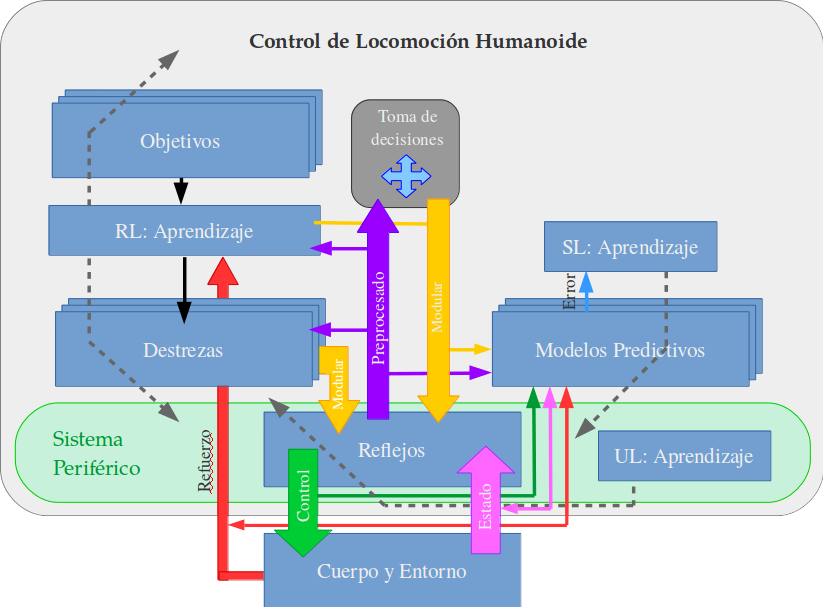
\includegraphics[width=1.0\textwidth]{images/ObjetivoGeneral.png}
  \caption{Estructura general de emergencia y aprendizaje de locomoci\'on basada en cognici\'on y reflejos}
  \label{fig:ObjGen}
\end{figure}

%Importante: Resaltar el aporte del objetivo general en la ciencia.

Algunas aplicaciones recientes que muestran la importancia del trabajo sobre la problematica planteada son

(Geyer)
Sobre pr�tesis transfemorales se estudia la recuperaci�n del balance de la marcha utilizando un control NM~\cite{Thatte2015}, logrando una mayor robustez en la marcha comparado con los controladores de impedancia, los cuales se destacan en pr�tesis actuadas. Esta comparaci�n se realiza mediante simulaci�n y hardware, obteniendo como resultado una mejor comunicaci�n entre el usuario y la pr�tesis, pero al final se plantea que es necesario estudiar mejor dicha pol�tica de control analizando la marcha anormal de un amputado.

\cite{Dzeladini2016}(Ijspeert)
Dzeladini, F. et al., 2016. Effects of a neuromuscular controller on a powered ankle exoskeleton during human walking. In Proceedings of the IEEE RAS and EMBS International Conference on Biomedical Robotics and Biomechatronics. pp. 617

% Ademas de utilizar hipotesis de las neurociencias y la psicolog\'ia, la rob\'otica ahora es utilizada para pruebas de hipotesis propuestas por estas dos ciencias, dando por creado la neuro-rob\'otica.

% Limitaciones
% \begin{itemize}
% \item Generaci\'on de trajectorias: por seguimiento[Citas], CPG[Citas] o HZD[Citas], se requiere que la estructura mec\'anica tienda a moverse sobre ciclos l\'imites. Sistemas autonomos y no-autonomos implicaciones de sincronizaci\'on.
% \item Basados en ZMP son quasi-est\'aticos[Citas]
% \item Limitaci\'on de los actuadores[Citas]
% \item Limitacion del sistema sensorial[Citas]
% \item Robustez a perturbaciones y habilidades ganadas.
% \item Adaptaci\'on de nuevos movimientos ante cambios del entorno y su necesidad a desempe\~narse
% \item Energ\'eticamente ineficientes
% \end{itemize}

% \par En la generaci\'on de trayectorias el empleo de redes bio-inspiradas de algunos insectos y animales son implementadas a trav\'es de los Central Pattern Generators presentes en el Sistema Nervioso Central \cite{Ijspeert2008}. Estas CPGs que representan osciladores acoplados (ver Figura \ref{fig:cpg}.) suelen configurar sus par\'ametros mediante algoritmos de optimizaci\'on, un ejemplo se puede ver en \cite{Kim2009} en el cual se usa enjambre de part\'iculas o por medio de aprendizeje Hebbiano \cite{Righetti2006a} este aprendizaje es guiado por lo general por una capa de control superior, denominada algunas veces Mesencephalic Locomotion Region {\textbf(MLR)}\cite{Shahbazi2012}.\\
% \par Otro caso que toma encuenta la interacci\'on de los sensores y los actuardores (ver Figura \ref{fig:SensingThroughBody}) para la formaci\'on de los reflejos, es una capa por lo general auto-organizada y presenta un aprendizaje no supervisado \cite{Iida2006,Manoonpong2007}. Posterior a estos trabajos \cite{Marques2013}, demuestra cuatro hip\'otesis de como se forman los reflejos apartir de la actividad espont\'anea de los actuadores o m\'usculos del agente y luego de su formaci\'on es posible la emergencia de un comportamiento coordinado, finalmente esta configuraci\'on permite adaptar su control a deficiencias morfol\'ogicas. En este \'ultimo trabajo se hace evidente el uso de aprendizaje supervisado y no supervisado.\\
% \par Por otra parte el aprendizaje por refuerzo ha sido utilizado para dise\~nar controles basados en control \'optimo y control adaptativo\cite{Wang2012a}. Las metodolog\'ias de Q-Learning y Actor-Critic han sido utilizadas con resultados notorios \cite{Tedrake2004}, en el que un agente logra la marcha en veinte minutos de aprendizaje. Q-learning es utilizado para el robot de la figura \ref{fig:SensingThroughBody} en \cite{Iida2009a}\\

% Control Robusto e inteligencia artificial

% Posibles reflejos: 
% Control tobillo, torso postura y posicionamiento del pie.
% ZMP, CoM, CoP, FRI, tiempo de duracion de la fase y longitud de paso. Velocidad promedio.


% Deep Learning. Aprendizaje por refuerzo.

% Como implementar?

% Robustez, versatilidad y eficiencia energ\'etica
% Sobre robustez: redundancia por medio de multiestrategias, usando el control de torque en el tobillo, la postura del torso  y el posicionamiento del pie.  Redundancia en la representacion reflexiva mediante la implementaci\'on morf\'ologica.

% Sobre versatilidad: La capacidad de adaptaci\'on. Aprendizaje y en especial la capacidad auto-organizaci\'on. La representaci\'on de conceptos o principios del la locomoci\'on b\'ipeda mediante Deep Learning.

% Sobre la eficiencia-energetica: El proceso de optimizacion, ya sea mediante algoritmos evolutivos o en general bio-inspirados, buscando hasta donde, con las restricciones tecnologicas nos permiten lograr un agente bipedo inteligente. Para esto la co-evoluci\'on de las estructuras de control y morfol\'ogicas deben ser dise\~nadas al tiempo

% Evaci\'on de obst\'aculos (bajo nivel) y navegacion (alto nivel- representaci\'on espacio-tiempo modelado) como ejercicios de planeaci\'on. Reflexivo e intencional \cite{Madani2011}.

% Observadores morfol\'ogicos, propiocepci\'on

% Control modular por niveles (reflexiva, memoria de destrezas, predictiva, creativa por motivacion, decisiva).
% Estructura b\'ipeda (basada en el modelo de \cite{Song2015}).
% Comportamiento racional (maximizando su recompenza futura, "tratar de hacer las cosas correctas").
% Reflejos auto-organizados ().
% Caracter\'isticas cognitivas (aprender, adaptarse, predecir y recordar).
% Computacion morfol\'ogica (forma de la implementaci\'on mediante la estructura mecanica o neuronal).
% Emergencia de locomoci\'on robusta y vers\'atil (programacion automatica).

% Exsiten desde el punto de la locomoci\'on b\'ipeda miles de esfuerzos por generar robots humanoides y no humanoides que sean capaces de caminar[Citas] o correr[Citas]. Adem\'as de estos esfuerzos por generar estructuras mec\'anicas que puedan moverse e interactuar como los humanos, existen n\'umerosos esfuerzos que intentan comprender la biomec\'anica del cuerpo humano probando hipotesis de forma computacional[Citas].

% ASIMO, HRP4 y NAO, son robots basados inicialmente en el concepto del ZMP, que es un movimiento ineficiente, con muy baja robustez aunque es versatil.
% Caminata din\'amica pasiva
% RABBIT, MABEL y MARLO capaces de correr y caminar
% PETMAN

% Desde el punto de vista biomec\'anico, el entendimiento del control de dicho sistema ha incluido la necesidad de entender y estudiar el sistema nervioso, y ante esto las teorias coneccionistas que incluyen las neurociencias han entrado a aportar difrentes hipotesis para el entendimiento de la locomoci\'on humanoide. Al estudiar el sistema neuronal nervioso, numerosas hipotesis y definiciones de conceptos aparecen. Las caracteristicas cognitivas deben son modeladas por diferentes redes neuronales.

% \par Generalmente la caminata b\'ipeda se analiza partiendo de muchos supuestos, un supuesto com\'un es anclar el pie soporte durate la fase de soporte simple. Como se demostr\'o en el trabajo de \cite{Chevallereau2008}, la fase de soporte doble es resumida en una din\'amica instant\'anea discreta que suele ser obviada ya que solo es necesaria su energ\'ia cin\'etica antes del impacto. Por esto en la mayoria de los analisis de marcha la fase de soporte doble es omitida y al asumir simetr\'ia en la marcha, el analisis queda reducido a llevar el pie de balance de atr\'as hacia adelante.\\
% \par Explicada la marcha, \cite{Chevallereau2008} adiciona un grado de libertad adicional que representa la punta del pie y su giro respeto a los dedos. La fase soporte ahora tiene incluida una subfase en la cual es permitida la rotaci\'on del pie respecto a la punta del mismo. Es importante resaltar que esta subfase adiciona un grado de libertad no actuado, convirtiendo el problema en subactuado. En \cite{Tlalolini2011}, repiten el modelo pero esta vez en tres dimensiones, al igual que en su trabajo anterior, las trayectorias deben ser encontradas mediante optimizaci\'on en donde las funciones objetivo son minimizar torque y energ\'ia y maximizando velocidad y estabilidad. Una conclusi\'on de este trabajo es que la rotaci\'on del pie es necesaria para grandes velocidades y longitudes de paso.\\
% \par Sin embargo mirando de una forma m\'as general, las condiciones con las que el caminador llega a la fase de soporte doble, la siguiente pregunta surge: ¿C\'omo saber que las condiciones din\'amicas al terminar un paso cualquiera, es decir entrando en la fase doble, conducen a una estabilidad dinamica? Para responder esto el ZMP o FRI, permiten cuantificar de cierta forma la estabilidad d\'inamica, pero el robot debe conocer en todo momento estos valores de ZMP o FRI. De igual manera si la caminata fuera de balance est\'atico, el CoM deberia ser la informaci\'on que el robot deberia conocer en cada momento de su marcha.\\
% \par Tomando como inspiraci\'on los seres vivos b\'ipedos, es sabido que ninguno realiza c\'alculos de ZMP, FRI o CoM para moverse bajo el r\'egimen de marcha b\'ipeda. Sin embargo desde el punto de vista de la computaci\'on morfol\'ogica \cite{Hauser2012a}, la alta riqueza no-lineal presente en el sistema estructural morfol\'ogico en conjunto con  su sistema neuronal, demuestra que  el cuerpo de un bipedo natural presenta una fuerte capacidad de computo. Aunque no sea consiente de ello, estos c\'alculos pueden ser materializados a traves de los circuitos de reflejos que estan presenetes en la capas sensormotrices las cuales han sido coevolucionadas con su morfolog\'ia y son esenciales en el control del caminador.\\
% \par Adem\'as de los reflejos de equilibrio y balance, flexi\'on y extensi\'on, debe existir otros reflejos adicionales de orden superior que representen en tiempo real diversos estados, acciones e intensiones de marcha sobre un b\'ipedo que permita asesorar las capas de control superior en cuanto a las acciones de control a tomar. Pregunta: ¿Es pisible almacenar distintos reflejos y circuitos neuronales que representen diferentes estados de marcha? ¿Deberian ser encontrados dichos reflejos y definidos? (O tal vez ya existen)\\
% \par Basado en (1) el sistema musculoesquel\'etico del ser humano y su sistema neuronal, (2) conociendo que estos sistemas son auto-organizado y que no existen dos iguales pero que tiene la misma estructura jerarquica, se plantea la siguiente pregunta de investigaci\'on: \\
% \emph{¿C\'omo y cuales son el conjuto de reflejos b\'asicos que necesitaria conocer un agente rob\'otico b\'ipedo, para lograr la emergencia de la locomoci\'on al nivel del control humano?}

% El ZMP utiliza el control the posicion del torso y el control del torque en el tobillo. El concepto de FRI intenta a\~nadir la posibilidad de griro del pie sobre alguno de los bordes del pie de apoyo.
% El HZP se ha utilizado en sistemas subactuados el control del torque en la cadera, rodillas y torso.
% El CPG requiere de un criterio de estabilidad externo y por lo general un control por modelo inverso.
% El posicioneamiento del pie, caracteriza una zona de posible descarga de la pierna que se balancea sobre la cual el caminador es capaz de regularse para no caer.

% Ciencias naturales: (1) Percepcion Sensar-Interpretar, (2) Accion Mover-Afectar y (3) Aprendizaje Adaptar-Evolucionar.

% Modelo del sistema $\dot{x}\,=\,f(x,u,t,\epsilon_x)$ y Modelo de observaci\'on $y\,=\,f(x,u,t,\epsilon_y)$.

% Distinci\'on entre \emph{skills and abilities}, habilidades son caracteristicas predeterminadas geneticamente que affectan el desempe\~no del movimiento como agilidad, coordinacion, fuerza y flexibilidad. Las habilidades son diferenciadas de las competencias en el sentido de que las competencias son aprendidas, mientras que las habilidades son el producto de la gen\'etica y el aprendizaje. Los skills son un nivel de experticia o alto grado de competencia para ejecutar una determinada tarea, mientras que las abilities son parte de los rasgos o caracteristicas individuales que afectan la capacidad de que el agente se vuelva h\'abil, talentoso o diestro cuando se aprende una nueva tarea motriz.

% Se propone necesidades de la robotica actual Benchmars y destrezas 3., 6.\cite{Torricelli2015}
% Un benckmark de locomocion bipeda es propuesto en una encuesta sobre las necesidades que presenta los investigadores actuales de humanoides, wearable robots y humanos. El interes de comprara desempe\~nos de direrentes tecnologias y estararizacion y regulariciacion de precesos en la inclucion del mercado. 
% FIgura 2. concepto general del benckmark
% Figura 4. Destrezas motoras consideradas para el benckmark

% ("El mejoramiento de una tarea puede estar dado por prueba-y-error o por la inferencia de datos percibidos y previas expreriencias" mejorar de forma interna mediante modelos de prediccion ¡hay quemejorar el sistema sensorial de la robotica!, mediante un mejor uso de la informacion sensorial) inspirado de \cite{Andre2015}

%(Proponer Plasticidad de la sinapsis con matrices esparsidas como en Deep Learning, para encontrar arquitecturas simples) \cite{Steingrube2011}

% Simspark para los datos del campeon de 2013 \cite{Shafii2015}

%deteccion de caida predictor con modelo, por data-driven o heuristicas \cite{Paiman2016}

%Procesos congintvos e inclusion de la nocion del tiempo\cite{Maniadakis2014}
% Modelos de tiempo y procesos cognitivos hasta ahora recientemente considerados, incluyen los aspectos temporales de la conciencia, integrando el tiempo en diffrentes modleos de capacidades percepto-motrices como la memoria la atencion, el planeamiento de acciones y la toma de decisiones.Se toman dos modelos, el primero es el "enfoque dedicado" que asume una metrica explicita del tiempo y el segundo que incluye explicaciones intrinsecas que describe al tiempo como una propiedad general y heredada de la dinamica neuronal.

%Por \'ulitimo se argumenta que los aspectos temporarles de la cognicion permiten integrar las otras propiedades cognitivas como: Memoria, aprendizaje, razonamiento, planeacion, action, comunicacion y atencion

\section{Hacia cognici\'on y reflejos encarnado}
\label{sec:hacia}
% Russell en espanol (1) "...the first robotic embodiment..." es "...el primer robot construido ..."
% Russell en espanol (2) "...are physical embodiments..." es "...son una manifestacion fisica ..."
% Russell en espanol (3) "...provides a natural embodiment of Ockham's razor..." es "...incluye de forma natural la navaja de Ockham ..."
% Russell en espanol (4) "...the first program to embody..." es "...el primer program que incorporo ..."
% Russell en espanol (5) "...it was to embody general knowledge of the world..." es "...manejaba el conocimiento general del mundo ..."
% Russell en espanol (6) "...agent programs that embody the principles..." es "...programas para agentes que encarnan los principios ..."
% Russell en espanol (7) "...that comes fairly close to embodying the declarative ideal..." es "...que esta bastante relacionada con abarcar el ideal declarativo ..."

La encarnacion permite el calculo distribuido de reducciones dimensionales que deben irse adaptando con el fin de mejorar la capacidad predictiva del ajente y con esto acelerar el proceso de aprendizaje y optimizacion de las tareas que realiza.

Problema abierto Busqueda de restriciones virtuales de forma on-line \cite{Grizzle2014}. 

hipotesis como heuristica para aprender mas rapido de trabajos como el de \cite{Kuo2001}.

Se debe caracterizar mejor la fase de doble soporte \cite{Grizzle2014}, esto seria una aplicacion para extraccion de caracteristicas analizando las se\~nales sensormotrices.

%Justificacion: Las politcas de destrezas y conocimiento se tiene que heredar atraves de una condificacion en el adn o mediante apredizaje con maestre usando imitacion. PI$2$ Policy improvement with path integrals for RL. Predicion de fallas con DMP-ASM!!!. Sensor Data mining  con ASM para encontrar causalidades, reduccion de representacion, extraccion de caracteristicas. Creacion automatica de modelos de comportamiento!!!. Exploracion de datos masivos por ejempo de la RoboCup.

El trabajo de marquez con iida pero aplicado a un modelo SMA hacia la caminata figura 2.9 \cite{HauserS2013}. ""Se puede aplicar para la locomocion en general""


\section{Algunas aplicaciones y motivaciones}
\label{sec:motivaciones}

% Aplicaciones e impacto en: rehabilitacion neuromotora, mejoramiejto del desempe\~no de atletas, o en la reproduccion de habilidades o destrezas humanas en sistemas artificiales comk robots.
% Automatizacion de tareas y optimizacion de las mismas

% aplicaciones e impacto en: rehabilitacion neuromotora, mejoramiejto del desempe\~no de atletas, o en la reproduccion de habilidades o destrezas humanas en sistemas artificiales comk robots.

% Dise\~no de caracteres o personajes de video juegos

% tareas compu3stas como caminar y alcanzar ojetos al mismo tiempo\cite{Moro2012}.

%parte de la metodolog�a
M\\
La combinaci�n de aprendizaje por imitaci�n y RL, denominado \emph{aprendizaje de principiante}, se caracteriza por la necesidad de un profesor y la practica realizada por el aprendiz. Es posible a partir de las demostraciones encontrar �ptimos locales que nos permitan tomar las demostraciones como pol�ticas iniciales de partida. Muchas veces las demostraciones humanas a humanoides deben ser adaptadas teniendo en cuenta las diferencias cinem�ticas entre el profesor y el robot. Otras veces el profesor controla directamente el robot  poder obtener una demostraci�n.


    
\chapter{Objetivos}
\label{chap:objs}

\section{Objetivo General}
\label{sec:objGen}
Proponer una metodolog�a para analizar y organizar la informaci�n procedente de la comunicaci�n entre el entorno y el cerebro a trav�s del lazo sensoriomotor, que permita extraer caracter�sticas naturales de locomoci�n de comportamientos ya aprendidos, con el fin de formar modelos internos que permitan estructurar controladores y estimadores del comportamiento de su morfolog�a e interacci�n con el entorno de forma predictiva.

\section{Objetivos Espec�ficos}
\label{sec:objEsp}

\begin{itemize}
\item Construir un modelo computacional de un humanoide con un sistema NMS, sobre el cual se pueda aprender comportamientos por auto-organizaci�n y demostraci�n, con la finalidad de formar un generador de muestras estadisticas, de comportamientos humanoides para analizar.
\item Construir un controlador jer�rquico, que aprenda modelos internos del lazo sensoriomotor y que mejore su desemple�o a medida que interact�e con su entorno.
\item Proponer un metodo de transferencia del controlador NMS a una arquitectura humanoide
%\item Utilizar un modelo del sistema NMS para representar el lazo sensoriomotor de un humanoide, sobre el cual se implemente estrategias de control de comportamientos coordinados auto-organizado o aprendidos por demostraci�n que cumplan el objetivo de un comportamiento.
%\item Extraer la funci�n de costo mediante IRL de comportamientos aprendidos y buscar una estrategia �ptima local del comportamiento aprendido mediante RL.
%\item Proponer modelos neuronales sobre el NMS que permitan representar modelos probabil�sticos del comportamiento del humanoide, que funciones como predictores de las acciones y estimadores del entorno.
\end{itemize}

    \chapter{Metodolog�a}
\label{chap:metho}

\section{La maquinaria por debajo}
\label{sec:maquinaria}
Para lograr el objetivo general, en la metodolog�a se propone utilizar el modelo NMS de Geyer~\cite{Geyer2010} extendido en~\cite{Song2015,Dzeladini2014}, como representaci�n de la planta real del humanoide a estudiar. Existe varias ventajas de tomar ese modelo: (1) Desde el punto de vista de la computaci�n morfol�gica, la complejidad de la se�al de control, como se demostr� en~\cite{Ghazi-Zahedi2015a}, permite simplificar el espacio del estado-acci�n, imponiendo adem�s restricciones naturales presentes en el cuerpo humano y explotando la riqueza din�mica natural de la auto-estabilizaci�n de algunos comportamientos mediante la \emph{m�rfosis} del sistema; (2) La implementaci�n de diferentes tipos de retardos sobre diferentes \emph{pathways}, permite formar acciones de control reactivas y otras de control predictivas, estas �ltimas requieren de un mayor c�mputo y un mayor tiempo, que son necesarios para tomar una decisi�n m�s elaborada. Esta caracter�stica constituye el fundamento morfol�gico de un control jer�rquico; (3) Aprovechando el modelo extendido de~\cite{Song2015}, la estructura jer�rquica permite diferentes tipos de movimientos como caminar, correr y transiciones de velocidades. Los tres bajo diferentes tipos de terrenos. Estos ser�n ejemplos demostrativos de movimiento, �tiles para el aprendizaje; (4) Aprovechando el modelo extendido de~\cite{Dzeladini2014} de la capa de CPGs, donde se permite modular los reflejos y formar predicciones de la interacci�n, adem�s de guardar dichas configuraciones de los CPGs como modelos predictivos. Esto ser� importante para practicar el \emph{ensayo mental}\footnote{mental rehearsal} y dar una forma estructurada a los modelos internos. 

La implementaci�n del modelo de Geyer, propuesto en~\cite{Dzeladini2014}, tiene una librer�a del sistema NMS desarrollada en C++ y es f�cil acoplar a un motor f�sico de din�mica multicuerpo. En este caso para el motor f�sico, las librer�as RDBL desarrolladas por~\cite{Felis2016}, de los algoritmos de~\cite{Featherstone2008} que incluyen un modelo de contacto e impacto con fricci�n~\cite{Uchida2015}, desarrolladas en C++ con extensi�n a Python a trav�s de Cython, son escogidas por la versatilidad del c�digo y su extensi�n para la optimizaci�n con GPU mediante CUDA a traves de Eigen 3~\cite{Guennebaud2010}.

% modelo de friccion, por que python?, por que C++, por que CUDA? visualizacion como post-proceso

% NOVEDAD: direcci�n sobre el modelo NMS, musculos en adicionales del pie
% NOVEDAD: usar DMPs en las restricciones virtuales en el controlador HZD
% NOVEDAD: modelos de SLIP y LIPM con HZD
% NOVEDAD: exploraci�n de la representaci�n de caracter�sticas en la funci�n de recompensa.

%Probability is about modeling uncertainty in the world.
%Inference is about learning properties of the world from data that we observe.
%Computation is needed to automate probabilistic analysis and inference, especially to handle massive data sets.
%Sterotypical movements enable prediction and statistics.
%For every movement skill, we associate motor and perceptual variables and theit statistics over time.
%This information, represented in memory as ASM, can be used in error corretion, pattern completion, switching and abort behaviors 

\section{La piedra angular de adaptaci�n: B�squeda de pol�ticas}
\label{sec:piedra}
Para la b�squeda de la pol�ticas mediante RL Rob�tico, configurar el algoritmo adecuado de RRL, requiere de pruebas con diferentes elecciones. Por el problema espec�fico del humanoide acoplado a un sistema NMS, solo al final de las pruebas se sabr� cu�l combinaci�n es la m�s adecuada. Por lo tanto especificar la configuraci�n del algoritmo de RRL, es un resultado que debe ser encontrado. La representaci�n de la pol�tica ser� mediante redes neuronales (ANNs), primitivas de movimiento din�micas (DMPs)\footnote{Las PMP tambi�n son una opci�n que se estudiar�} y Osciladores morfados (MOs), estos �ltimos~\cite{Ajallooeian2013} son una generalizaci�n de los DMPs r�tmicos y los CPGs. Un algoritmo RRL tiene por lo general tres ingredientes: un paso de evaluaci�n de pol�ticas, otro paso de mejoramiento o actualizaci�n de pol�ticas y un m�todo de exploraci�n. Es posible configurar dichos ingredientes utilizando diferentes estrategias~\cite{Kober2013,Deisenroth2013}. Los tres ingredientes ser�n claramente estudiados, teniendo en cuenta: (1) Por \emph{evaluaci�n de la pol�tica}, donde la evaluaci�n puede ser cada paso o cada episodio, o donde se puede utilizar las t�cnicas de \emph{diferencias temporales} (TD); (2) Por \emph{actualizaci�n de la pol�tica}, en donde se debe elegir entre algoritmos basados en: el \emph{gradiente de la pol�tica}, el algoritmo EM\footnote{Expectaci�n-Maximizaci�n}, las m�tricas de Informaci�n (IT), las integrales de camino ($PI^2$) y la optimizaci�n estoc�stica; y la �ltima (3) Por \emph{estrategia de exploraci�n}, que tiene a�n m�s posibilidades, las cuales pueden funcionar en conjunto, dando m�ltiples combinaciones posibles. Estas son: (i) \emph{espacio de la perturbaci�n}, sobre el espacio de acci�n o el espacio de par�metros, en el �ltimo se puede estructurar el ruido y trabajar un nivel superior de aprendizaje de pol�tica; (ii) \emph{escala de tiempo}, nuevamente esta por paso o por episodio, en el primero se puede evitar los m�nimos locales y en el segundo, las actualizaciones de las pol�ticas resultan m�s confiables; (iii) \emph{distribuci�n de ruido}, en donde se usa matrices de correlaci�n basadas en m�todos de segundo orden, ac� el m�todo de \emph{Covariance Matrix Adaptation} (CMA) ser� estudiado por sus resultados; y (iv) \emph{actualizaci�n de la distribuci�n del ruido} donde se puede variar las tasas de exploraci�n y utilizar m�tricas de entrop�a relativa a medida que itera el algoritmo.

En cuanto al problema de volver el RRL tratable, los retos en la metodolog�a son: 
\begin{enumerate}
\item El \emph{problema de la dimensionalidad} que se enfrentar� mediante tres ideas: (1) la representaci�n de pol�ticas parametrizadas y estructuradas, utilizando MOs para movimientos r�tmicos y DMPs para movimientos discretos, aplicados al nivel de activaci�n muscular como representaci�n de las pol�ticas; (2) las sinergias musculares propuestas y la capacidad de c�mputo del MC en el modelo NMS presentado en~\cite{Song2015} como la reducci�n de la dimensionalidad, la simplificaci�n de la se�al de control y el manejo de variables latentes; y (3) la b�squeda local partiendo de ejemplos demostrativos. 
\item La \emph{exploraci�n cuidadosa}, mediante las cuatro opciones de estrategias de exploraci�n descritas anteriormente, busca pol�ticas que no sean nocivas o destructivas para la estructura del humanoide. El punto clave aqu�, es una exploraci�n local que tambi�n contribuye para tratar el problema de la dimensionalidad.
\item La \emph{eficiencia estad�stica}. En este punto el manejo eficiente de grandes cantidades de datos, procedentes de la informaci�n del lazo sensoriomotor al interactuar, se logra de la formaci�n de modelos probabil�sticos internos, que representan modelos directos locales, estimadores de estado, modelos de recompensa, predicciones de fallos ante perturbaciones y otros m�s, que permiten la capacidad cognitiva de realizar ensayos metales produciendo un manejo eficiente de los datos y una eficiencia estad�stica que reduce el n�mero de muestras. El uso de \emph{mini-batches} y un manejo adecuado de los datos de muestra, permite aproximar el problema a variables \emph{i.i.d}, que habilitan el uso de los m�todos de aprendizaje supervisado del ML.
\end{enumerate}

% Funci�n de recompensa seg�n tipos de tareas dependiendo peri�dicas o discretas, forma parametrizable y basada en Bolza, codificaci�n de la tarea. Representaci�n de la intenci�n del agente
% La se�al de recompensa es una representaci�n compacta de la intenci�n del humanoide y contiene informaci�n que lleva al agente hacia sus objetivos. Ese conocimiento suele ser transferible. Generalmente es dada por el programador, el cual tiene experiencia en el problema o es derivada de la experiencia del agente. Recompensa descontada, tiempo finito o recompensa acumulada promedio. Funci�n no-lineal de recompensa, Bayesian IRL, Maximum entropy IRL y PI$^2$. El cuello de botella. Expertos con incompletas e imperfectas demostraciones. Una funci�n de recompensa sirve para representaciones portables de comportamientos, permitiendo la generalizaci�n a nuevos dominios. Usando DNN se pierde la estructura dise�ada a mano por los algoritmos IRL tradicionales
La funci�n de costo o recompensa inicialmente se probar� como una se�al dispersas sobre una estructura de Bolza tradicional, no obstante es necesario usar el \emph{Aprendizaje por Refuerzo Inverso} (IRL) o \emph{Control �ptimo Inverso} (IOC), el cual encuentra la funci�n de recompensa, a partir de ejemplos demostrativos que son asumidos frecuentemente como �ptimos. En la se�al de recompensa se codifican los comportamientos y la principal ventaja de su extracci�n es, que las funciones son transferible a distintas morfolog�as, sin embargo existe el inconveniente de que muchas funciones de costo representan el mismo comportamiento, con lo cual la soluci�n del problema de IRL se complica. Otra ventaja es que dependiendo de la se�al de recompensa, el aprendizaje de una tarea puede ser notoriamente acelerado. Para aprender una buena se�al de costo se utilizar�: (1) para la \emph{representaci�n de la funci�n de recompensa}, combinaciones lineales de funciones caracter�sticas dependientes �nicamente del estado y tambi�n, redes neuronales profundas (DNN) las cuales son una representaci�n no lineal de las caracter�sticas; (2) los \emph{algoritmos} de: ${PI}^2$ basado en DMP, \emph{Guided Cost Learning} basado en una estructura de costo DNN y \emph{M�xima Entrop�a}, capaz de enfrentar problemas de alta dimensi�n de modelos dinamicos desconocidos con un numero bajo de ejemplos. 

Para la b�squeda por RL, la funci�n de costo o recompensa, se propondr� de diferentes formas: (1) manual de forma \emph{dispersa}, (2) mediante \emph{aprendizaje por refuerzo inverso} (IRL) del ejemplo sub-�ptimo demostrativo de locomoci�n, (3) mediante IRL de la caminata del modelo NMS de Geyer.

%parte de la metodolog�a
La combinaci�n de aprendizaje por imitaci�n y RL, denominado \emph{aprendizaje de principiante}\footnote{Apprenticeship Learning}, se caracteriza por la necesidad de un instructor y la practica realizada por el aprendiz. Es posible a partir de las demostraciones encontrar �ptimos locales, que nos permitan tomar las demostraciones como pol�ticas iniciales de partida. Muchas veces las demostraciones humanas a humanoides deben ser adaptadas teniendo en cuenta las diferencias morfol�gicas entre el instructor y el robot. Otras veces el instructor controla directamente el robot, para poder crear una demostraci�n v�lida. En este caso las demostraciones partir�n de controles humanoides reconocidos y comportamientos auto-organizados, que no necesariamente se basan sobre modelos NMS pero que si tienen una estructura humanoide, de trabajos anteriores.

La estructura esquem�tica del entorno-cerebro y el lazo sensoriomotor est� representada en la figura \ref{fig:ObjGen}, en donde se exhibe, c�mo el lazo sensoriomotor se acopla al cerebro por un lado y por el otro al entorno. El entorno incluye el cuerpo del humanoide. El lazo sensoriomotor es el sistema perif�rico representado por parte del sistema NMS, espec�ficamente la parte que controla al sistema m�sculo-esquel�tica por medio de la din�mica neuronal de la activaci�n del modelo muscular de Hill, los reflejos y los modelos de CPGs. Fisiol�gicamente desde las se�ales eferentes-aferentes, la m�dula y hasta antes del \emph{tronco encef�lico}\footnote{brainstem}. Se puede apreciar, que tiene diferentes mecanismos de adaptaci�n: (1) aprendizaje auto-organizado, (2) aprendizaje supervisado y (3) aprendizaje por refuerzo. El aprendizaje de principiante se realiza utilizando una combinaci�n de los tres mecanismos anteriores.

\begin{figure}[!htb]
  \centering
  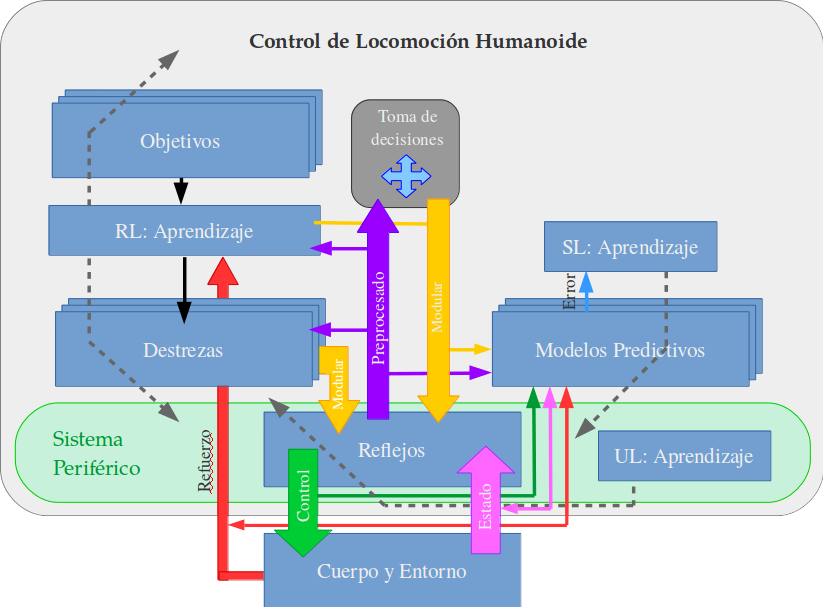
\includegraphics[width=1.0\textwidth]{images/ObjetivoGeneral}
  \caption[Estructura general de emergencia y aprendizaje]{Estructura general de emergencia y aprendizaje de locomoci\'on basada en cognici\'on y reflejos}
  \label{fig:ObjGen}
\end{figure}

\section{Objetivo 1: Construcci�n del modelo humanoide}
\label{sec:obj1}
Dos casos de estudio: (1) el primero la caminata en el plano con control de direcci�n para cumplir objetivos de posici�n, partiendo de ejemplos demostrativos; y (2) el otro consiste en comportamientos auto-organizado de mantener el equilibrio mediante la colocaci�n del pie y la utilizaci�n de los brazos, en un ambiente pre-estructurado. Con los casos de estudio anteriores mediante \emph{aprendizaje de principiante} se forma un conjunto de datos que permitir� el desarrollo del comportamiento y el control del humanoide, mejorando su desempe�o a trav�s del ensayo y error.

% Proponer una estrategia que evolucione los controladores de locomoci�n humanoide actuales basados en ZMP hacia una locomoci�n m�s natural
Mediante el primer caso de estudio, se utiliza una caminata basada en ZMP y HZD similar a la de~\cite{Wang2012}. Para tomar la estructura de control y locomoci�n propuestas, como punto de partida de un ejemplo sub-�ptimo demostrativo de locomoci�n. Esto con el fin de que el sistema NMS aprenda dicho comportamiento y a partir de ello, busque mediante RL una soluci�n �ptima local, que mantenga el balance din�mico pero que elimine la restricci�n del ZMP, elimine la flexi�n de rodilla y permita la rotaci�n del pie, en busca de una locomoci�n m�s natural. En este paso la optimizaci�n que requiere las \emph{restricciones virtuales}, se har� mediante DMPs como un caso especial del los MO. Otra ventaja de usar las restricciones virtuales es que a trav�s de ellas se puede probar otros controladores cl�sico basados en IPM, LIPM, SLIP. El ultimo constituye un \emph{template} muy importante para el estudio de la locomoci�n con extremidades y es un punto de partida para los ensayos mentales.

Mediante otro caso de estudio, basado en el trabajos de \emph{Playful Machines} de~\cite{Der2012,Martius2013,Der2015}, en donde se explora la formaci�n de objetivos sobre la excitaci�n del lazo sensoriomotor, para producir emergencia de comportamientos que son auto-organizados en el sistema NMS, se analizar� el caso de ponerse en pie y mantener el equilibrio, ya sea con ayuda de los brazos o mediante la colocaci�n del pie. La maximizaci�n de la informaci�n predictiva ser� la clave en la exploraci�n de estos comportamientos. En este paso, tal y como se obtuvo en~\cite{Martius2014}, a trav�s de ciertos patrones deseados de se�al sensorial, se buscar� los movimientos deseados. Aqu� el ejercicio de transferir el comportamiento al sistema NMS propuesto, es por medio de una estructura auto-organizable presentada sobre el sistema NMS de~\cite{Marques2014}.

\section{Objetivo 2: Modelos internos del lazo sensoriomotor}
\label{sec:obj2}
Para explorar los mecanismos de corto y largo plazo presentes en el sistema NMS y su relaci�n con la estructura de controladores jer�rquicos, se utiliza el segundo caso de estudio del objetivo anterior. Utilizando el control b�sico de equilibrio auto-organizado, que se obtuvo del an�lisis del caso, donde la postura (incluyendo la ayuda de las extremidades superiores) y colocaci�n del pie, se controlan inicialmente por una capa de bajo nivel constituida por reflejos. En este segundo objetivo se construye un controlador jer�rquico con dos capas adicionales. La primera, una capa intermedia de la colocaci�n del pie y el balance donde se puede controlar a voluntad, mediante un proceso no reflexivo que implica un mayor tiempo de c�mputo. Y en una �ltima capa, la estrategia de desplazamiento general en el entorno es construida, con la finalidad de alcanzar un lenguaje de comunicaci�n entre el entorno y robot, mediante peque�as misiones de desplazamiento y paso de obst�culos. El dise�o de la se�al de recompensa de implementar� de forma jer�rquica y modular utilizando las t�cnicas de IRL. Las capas intermedia y superior deben estar dotadas de modelos internos del cerebro-entorno.

Para la implementaci�n de los \emph{ensayos mentales}, el lazo sensoriomotor ser� representado por un modelo gr�fico propuesto por~\cite{Ay2015}, con diferentes tipos de arquitecturas del Deep Learning. Algunas de ellas, de inter�s en esta investigaci�n ser�n evaluadas: Deep NNs, LSTM, Deep RBM, Deep Belief Networks (DBN), para aproximar modelos de distribuciones presentes en un modelo bayesiano, como se especula en~\cite{Goodfellow2016}. Una ventaja de estos modelos es que se puede ajustar el tama�o de la red a mediada que el comportamiento aumenta como es explicado en~\cite{Montufar2015}. La integraci�n de los comportamientos aprendidos en el primer objetivo, implementados sobre un �nico controlador, proponiendo un control jer�rquico, que module las tareas dependiendo de una comunicaci�n b�sica entre el entorno y el controlador. 

\section{Objetivo 3: Metodolog�a de transferencia del controlador}
\label{sec:obj3}
En el �ltimo de los objetivos, se desea analizar las estructuras de los modelos internos que constituyen los controladores de los objetivos anteriores y comprarlos con los originales de ZMP-HZD para proponer criterios de control m�s parecidos a los de la locomoci�n humana. La transferencia a un humanoide con NMS virtual mediante restricciones virtuales y HZD, es el paso final para cerrar.

    
\chapter{Cronograma y Actividades}
\label{chp:chrome}


\section{Actividades}
\label{sec:activities}

Acontinuaci\'on se enumera las actividads relacionadas con cada objetivo:

\begin{itemize}
\item \textbf{Obj 0}
  \begin{itemize}
  \item \textbf{Act 0.1} Revision bibliografica
  \item \textbf{Act 0.2} Documentacion y escritura
  \item \textbf{Act 0.3} Integracion de librerias MNS y RBDL
  \item \textbf{Act 0.4} Desarrolo de modelos individuales
  \item \textbf{Act 0.5} Pruebas de RL
  \item \textbf{Act 0.6} Pruebas de IRL
  \end{itemize}
\item \textbf{Obj 1}
  \begin{itemize}
  \item \textbf{Act 1.1} Caso de estudio 1. Ejemplos de controlador ZMP-HZD
  \item \textbf{Act 1.2} Aprendizaje por demostracion Caso 1
  \item \textbf{Act 1.3} Caso de estudio 2. Equilibrio y balance desde la auto-organizacion
  \item \textbf{Act 1.4} Aprendizaje por demostracion Caso 2
  \end{itemize}
\item \textbf{Obj 2}
  \begin{itemize}
  \item \textbf{Act 2.1} Desarrollo de modelos internos: prueba de arqutectura MLP
  \item \textbf{Act 2.2} Desarrollo de modelos internos: prueba de diferentes arquitecturas
  \item \textbf{Act 2.3} Dise\~no de controladores jerarquicos: Prebas sobre la se\~nal de recompensa
  \end{itemize}
\item \textbf{Obj 3}
  \begin{itemize}
  \item \textbf{Act 3.1} Transferencia de controladores
  \item \textbf{Act 3.1} Metodologia de dise\~no de controladores usando NMS virtual
  \end{itemize}
\end{itemize}

\section{Cronograma}
\label{sec:chrone}

Acontinuaci\'on se relaciona las dependencias temporales de cada actividad:

%\begin{landscape}
\begin{table}[!hbt]
  \centering
  \definecolor{RoyalBlue}{rgb}{0.0, 0.14, 0.4}
  \definecolor{OliveGreen}{rgb}{0.2745, 0.4196, 0.2392}%{0,0.6,0}%{0.33, 0.42, 0.18}
  \definecolor{Maroon}{rgb}{0.5, 0.0, 0.0}
  \begin{ganttchart}[
    y unit title=0.4cm,
    y unit chart=0.5cm,
    vgrid, hgrid,
    time slot format=isodate-yearmonth,
    compress calendar,
    title/.append style={draw=none, fill=RoyalBlue!50!black},
    title label font=\sffamily\bfseries\color{white},
    title label node/.append style={below=-1.6ex},
    title left shift=.05,
    title right shift=-.05,
    title height=1,
    bar/.append style={draw=none, fill=OliveGreen!75},
    bar height=.6,
    bar label font=\normalsize\color{black!50},
    group right shift=0,
    group top shift=.6,
    group height=.3,
    group peaks height=.2,
    bar incomplete/.append style={fill=Maroon},
    compress calendar
    ]{2016-9}{2018-6}
    \gantttitlecalendar{year} \\
    \ganttbar{Act. 0.1}{2016-9}{2018-2} \\
    \ganttbar{Act. 0.2}{2016-9}{2018-2} \\
    \ganttbar[progress=90]{Act. 0.3}{2016-9}{2016-11} \\
    \ganttbar[progress=77]{Act. 0.4}{2016-9}{2016-11} \\
    \ganttbar[progress=94]{Act. 0.5}{2016-9}{2016-11} \\
    \ganttbar[progress=95]{Act. 0.6}{2016-9}{2016-11} \\
    \ganttbar[
    progress=95,
    bar progress label font=\small\color{OliveGreen!75},
    bar progress label node/.append style={right=4pt},
    bar label font=\normalsize\color{OliveGreen},
    name=pp
    ]{Obj. 0}{2016-9}{2016-11} \\
    \ganttset{progress label text={}, link/.style={black, -to}}
    \ganttgroup{Obj. 1}{2016-12}{2017-5} \\
    \ganttbar[progress=4, name=T1A]{Act. 1.1}{2016-12}{2017-02} \\
    \ganttlinkedbar[progress=0]{Act. 1.2}{2017-03}{2017-5} \\
    \ganttbar[progress=4, name=T1B]{Act. 1.3}{2016-12}{2017-02} \\
    \ganttlinkedbar[progress=0, name=T1D]{Act. 1.4}{2017-03}{2017-5} \\
%    \ganttbar[progress=4, name=T1A]{Task A}{2016-12}{2017-04} \\
%    \ganttlinkedbar[progress=0]{Task B}{2017-07}{2017-12} \\
%    \ganttbar[progress=4, name=T1C]{Task C}{2016-12}{2017-04} \\
    \ganttgroup{Obj. 2}{2017-3}{2017-10} \\
    \ganttbar[progress=4, name=T2A]{Act. 2.1}{2017-3}{2017-4} \\
    \ganttlinkedbar[progress=0,]{Act. 2.2}{2017-05}{2017-8} \\
    \ganttbar[progress=4, name=T2B]{Act.2.3}{2017-6}{2017-10} \\
%    \ganttbar[progress=15, name=T2A]{Task A}{2017-01}{2017-09} \\
%    \ganttlinkedbar[progress=0]{Task B}{2017-10}{2017-12} \\
    \ganttgroup{Obj. 3}{2017-11}{2018-1} \\
    \ganttbar[progress=4, name=T3A]{Act. 3.1}{2017-11}{2018-1} \\
    \ganttbar[progress=4, name=T3B]{Act. 3.2}{2017-11}{2018-1} \\
%    \ganttbar[progress=0]{Task A}{2017-05}{2017-08}
    \ganttset{link/.style={OliveGreen}}
    \ganttlink[link mid=.8]{pp}{T1A}
    \ganttlink[link mid=.8]{T1B}{T2A}
    \ganttlink[link mid=.8]{T1D}{T2B}
    \ganttlink[link mid=.8]{T1B}{T2A}
    \ganttlink[link mid=.8]{T1D}{T2B}
%    \ganttlink[link mid=.159]{pp}{T2A}
  \end{ganttchart}    
  \caption{Cronograma del desarrollo de la metodolog\'ia}
  \label{tab:method}
\end{table}
%\end{landscape}

%    \include{cap0}
%    \include{cap2}
%    \include{cap3}
%\appendix
%    \include{apendice}
\backmatter
%    \conclusion{conclusiones}
%    \futurework{trabajofuturo}
%    \glossary{glosario}
%\nocite{*}
%    \bibliography{bibliografia}
\bibliography{\myreferences}
    %\printindex
\end{document}
